\documentclass[sigplan,10pt,review,anonymous]{acmart}
\settopmatter{printfolios=true,printccs=false,printacmref=false}
\setcopyright{none}
%\acmISBN{} % \acmISBN{978-x-xxxx-xxxx-x/YY/MM}
%\acmDOI{} % \acmDOI{10.1145/nnnnnnn.nnnnnnn}

% Packages {{{
\usepackage{hyperref}
\usepackage{amsmath}
\usepackage{amssymb}
\usepackage{bbm}
\usepackage{tikz}
\usetikzlibrary{calc}
\usetikzlibrary{graphs}
\usetikzlibrary{cd}
\usetikzlibrary{patterns}
\usepackage{bussproofs}
\usepackage{galois}
\usepackage{stmaryrd}
\usepackage{calc}
\usepackage{bbm}
\usepackage{soul}
\usepackage{booktabs}
% }}}

% Parameters {{{

\hyphenation{Comp-Cert}
\hyphenation{Comp-CertO}

% }}}

% Macros {{{

%\newtheorem{example}{Example}
%\newtheorem{definition}{Definition}
%\newtheorem{lemma}{Lemma}

\newcommand{\kw}[1]{\ensuremath{ \mathsf{#1} }}
\newcommand{\ifr}[1]{\mathrel{[{#1}]}}
\newcommand{\ifrw}[2]{\mathrel{[{#2} \Vdash {#1}]}}
\newcommand{\alt}{\ |\ } % use \mid instead
\newcommand{\bind}{\gg\!\!=}

\newcommand{\EC}{\kw{C}}
\newcommand{\simrel}{\kw{simrel}}

% Moves
\newcommand{\mcall}[3]{\kw{#1}({#2})@{#3}}
\newcommand{\pcall}[3]{%
  \underline{\mcall{#1}{#2}{#3}}%
}
\newcommand{\mret}[2]{{#1}@{#2}}
\newcommand{\pret}[2]{%
  \underline{\mret{#1}{#2}}%
}
\newcommand{\mretx}[3]{{#1}@{#2}/{#3}}
\newcommand{\pretx}[3]{%
  \underline{\mretx{#1}{#2}{#3}}%
}

\newcommand{\que}{\circ}
\newcommand{\ans}{\bullet}
\newcommand{\vref}{\sqsubseteq_\kw{v}}
\newcommand{\mext}{\sqsubseteq_\kw{m}}
\newcommand{\scref}{\preceq}

% Pointers for justified sequences %{{{

% Parameters
\newcommand{\pshift}{1.6ex}
\newcommand{\pcdist}{2.5}
\newcommand{\pcangle}{60}

% Pointer hook
\newcommand{\ph}[1]{%
  \tikz[remember picture]{\coordinate (#1);}}

% Pointer to
\newcommand{\pt}[1]{%
  \rule{0pt}{1.4em}%
  \tikz[remember picture, overlay]{
    \draw[->]
      let \p{dest} = (#1),
          \n1 = {ln(veclen(\x{dest}, \y{dest}) + 1)},
          \p1 = ($(0,0)+(0,\pshift)$),
          \p4 = ($(#1)+(0,\pshift)$),
          \p2 = ($(\p1)!\n1*\pcdist!-\pcangle:(\p4)$),
          \p3 = ($(\p4)!\n1*\pcdist!+\pcangle:(\p1)$) in
        (\p1) .. controls (\p2) and (\p3) .. (\p4);}}

%}}}

% }}}

\title{Refinement-Based Game Semantics for CompCert} %{{{

\author{J\'er\'emie Koenig}
\affiliation{Yale University}
\email{jeremie.koenig@yale.edu}

\author{Zhong Shao}
\affiliation{Yale University}
\email{zhong.shao@yale.edu}

%}}}

\begin{document}

\begin{abstract} %{{{
Since the introduction of CompCert,
researchers have been refining
its language semantics and correctness theorem,
and used them in
large-scale software verification efforts.
Meanwhile,
artifacts ranging from CPU designs to network protocols
have been successfully verified,
and there is interest in
making them interoperable
to tackle end-to-end verification
at an even larger scale.

To that end,
we believe that
a synthesis of existing research on
game semantics,
refinement-based methods, and
abstraction layers
has the potential to serve as a common theory
of certified components,
and that integrating CompCert to such a theory
is a critical goal.
However,
the requirements we have identified for
CompCert to be deployed in this context
are not met by any of its existing variants.

CompCertO is
a new extension of CompCert
which characterizes compiled program modules
in terms of their interaction with other components.
By extending the CompCert semantics
in a way that embraces relational reasoning,
we achieve this with only a minimal increase
in proof size.
\end{abstract}
%}}}

\maketitle

\section{Introduction} %{{{

% preamble {{{

The certified compiler CompCert \cite{compcert}
has represented a milestone
in terms of the scale at which software verification techniques
have been applied,
but most importantly
it has been used as a platform for other projects to build upon.
For instance,
verification tools have been created with soundness proofs
connecting to CompCert \cite{vst,verasco},
and it has been used as a component
in larger verification projects \cite{popl15}.

More broadly, over the past decade,
researchers have been able to formally verify the
total functional correctness
of various key components of computer systems,
including
%compilers \cite{compcert, vellvm},
operating system kernels \cite{sel4, popl15},
file systems \cite{fscq} and
processor designs \cite{safe}.
These achievements remain discrete, but
there is interest in rendering them interoperable,
as exemplified by the DeepSpec project \cite{deepspec}.
By using formal specifications as interfaces
between the correctness proofs of various components, %---
%showing that the requirements of one component
%are met by the guarantees of another ---
the researchers in DeepSpec hope to
verify composite systems
operating across many levels of abstraction.
%If successful,
%this would represent a deployment of formal methods
%at an unprecedented scale.

%}}}

\subsection{Refinement-based game semantics} %{{{

To enable this,
we are investigating
\emph{refinement-based game semantics}
as a common framework for
describing and reasoning about heterogenous systems.
Game semantics (\S\ref{sec:gamesem})
provides a highly flexible and expressive approach
to compositional semantics,
making it a plausible setting for this task.
By incorporating ideas from
the refinement calculus \cite{refcal}
and abstraction layers \cite{popl15}
into game semantics,
we hope to provide a framework
in which disparate verified artifacts
can be embedded and their correctness proofs combined.

%}}}

\subsection{Requirements for CompCert} \label{sec:compcertreq} %{{{

Given the central role CompCert has played
in the modern formal methods landscape,
its integration
should be a litmus test for any such effort.
Moreover, there is an abundance of research
seeking to make the correctness theorem of CompCert
more precise and compositional
\cite{qompcert,sepcompcert,compcompcert,compcerttso,compcertshm,compcertm},
which we can build upon to achieve that goal.

However, this new application of CompCert also
comes with its own challenges.
For the framework to be general,
it cannot be designed around CompCert itself.
It should be possible to reason about
C and assembly components that are part of
much more complex systems,
for instance
involving hardware components.
This excludes approaches to
per-module compilation correctness which are formulated in terms
of completed programs,
rather than characterizing a module's interactions
with its environment directly.

We believe that for our purposes
the compiler's correctness proof
should satisfy the following requirements:
\begin{enumerate}
\item \label{req:opensem}
  The semantics of the source and target languages
  should characterize the behavior of \emph{open} components
  in terms of their interactions with the rest of the program.
\item \label{req:opensim}
  The correctness theorem
  should go beyond refinement under a fixed notion of context, and relate
  the interactions of the source and target modules directly.
\item \label{req:openabs}
  The abstraction gap between C and assembly-level
  interactions should be formalized explicitly.
\item \label{req:linking}
  Some form of certified \emph{linking}
  should be provided as well as certified compilation.
\item \label{req:complexity}
  To facilitate integration into the official release,
  changes to the existing proofs of CompCert
  should be minimal.
\end{enumerate}
Each of these requirements is fulfilled
by some exisiting CompCert extension,
however none satisfies them all.

%With each step,
%the user can gain more confidence in the reliability of CompCert:
%existing work %testing the correctness of existing compilers
%has found fewer bugs in CompCert,
%compared to unverified alternatives \cite{csmith},
%and efforts to make CompCert's correctness theorem more realistic
%have uncovered and removed some of the few remaining bugs \cite{sepcompcert}.
%Much of this work has focused on making
%the correctness proof of CompCert more compositional,
%making it possible to prove properties about
%programs constructed from several independently compiled units,
%and to compositionally verify programs.

%}}}

\subsection{Contribution} %{{{

This paper introduces CompCertO,
the first extension of CompCert to tackle
all of these requirements simultaneously.

We generalize CompCert semantics
to express interactions between components (\S\ref{sec:sem}),
using \emph{language interfaces}
to describe the form of these interactions (\S\ref{sec:sem:open}),
and \emph{simulation conventions}
to relate the language interfaces
of the source and target programs (\S\ref{sec:sem:ref}).
The intended behavior of
multi-module programs is specified by a
\emph{horizontal composition} operator (\S\ref{sec:sem:linker}),
which is shown to be correctly implemented
by the existing linking operator for assembly programs.

To facilitate reasoning about
simulation conventions,
we define \emph{CompCert Kripke logical relations}
(CKLR, \S\ref{sec:cklr}),
which formalize the insight that
CompCert's memory transformations can be seen
as structure-preserving relations
over the CompCert memory model.
Among other uses,
CKLRs can be promoted to an endogenous
simulation convention for the $\mathcal{C}$
language interface.

As discussed in \S\ref{sec:passes},
the resulting conventions
cover most of CompCert's simulation proofs,
which can be updated with minimal effort.
But even in the case of more complex passes,
conventions can be defined
which capture the internal invariants
used by the existing simulation relations,
avoiding many sources of complexity found
in previous work.

In \S\ref{sec:simalg} we formalize the algebraic techniques
we use to compose the simulation proofs of the passes of CompCertO
into an overall forward simulation,
which serves as our compiler correctness theorem.
We describe how our framework
can be used to perform compositional compilation and verification,
and in \S\ref{sec:rw} we compare our results with related research.

[The public URL of the CompCertO repository is omitted
for the purposes of the double-blind review process
but has been provided in HotCRP alongside this submission.]

%}}}

%}}}

\section{Main ideas} \label{sec:mainideas} %{{{

\subsection{Principles for system construction} \label{sec:principles} %{{{

% preamble {{{

The goal of certified system design is
to create a formal description of
the system (the program) to be constructed,
while ensuring
that the system
will behave properly
through careful analysis.
To this end,
we assign
to a system description $p \in P$
a mathematical object $\llbracket p \rrbracket \in \mathbb{D}$
representing its behavior.
We will call the set $\mathbb{D}$ a \emph{semantic domain}.
In this section we elucidate
the structure and properties of $\mathbb{D}$
necessary to the process of builing
large-scale certified systems.

%}}}

\paragraph{Specifications and refinement} %{{{

System design starts with a set of requirements
on the behavior of the system to be constructed
(the specification).
These requirements do not capture every detail
of the eventual system,
but delineate a range of acceptable behaviors.

In refinement-based approaches,
programs and specifications are interpreted in the same
semantic domain $\mathbb{D}$,
which is equipped with a \emph{refinement} preorder
${\sqsubseteq} \subseteq \mathbb{D} \times \mathbb{D}$.
The proposition $\sigma_1 \sqsubseteq \sigma_2$
asserts that $\sigma_2$ is a refinement of $\sigma_1$,
and in particular a system description $p \in P$ is a correct implementation
of $\sigma \in \mathbb{D}$ when
$\sigma \sqsubseteq \llbracket p \rrbracket$.

%}}}

\paragraph{Compositionality} %{{{

Complex systems are built by assembling components
whose behavior is understood,
such that their interaction achieves a desired effect.
The syntactic constructions of
the language used to describe systems
correspond to the ways in which they can be composed.

To enable compositional reasoning,
a suitable model must provide an account of
the behavior of the composite system
in terms of the behavior of its parts.
For instance,
if the language contains a binary operator
${+} : P \times P \rightarrow P$,
then the semantic domain should be equipped with
a corresponding operation
${\oplus} : \mathbb{D} \times \mathbb{D} \rightarrow \mathbb{D}$
such that
$\llbracket p_1 + p_2 \rrbracket =
 \llbracket p_1 \rrbracket \oplus \llbracket p_2 \rrbracket$.

%}}}

\paragraph{Monotonicity} %{{{

Once a component has been shown to conform to a given specification,
we want to abstract it as a ``black box''
so that further reasoning can be done in terms of
the component's specification rather than its implementation details.
To support this,
we must establish that semantic composition operators
are compatible with refinement:
\[ \sigma_1 \sqsubseteq \sigma_1' \wedge
   \sigma_2 \sqsubseteq \sigma_2' \Rightarrow
   \sigma_1 \oplus \sigma_2 \sqsubseteq \sigma_1' \oplus \sigma_2' \,. \]
Suppose we have two components $p_1$ and $p_2$,
where $p_2$ relies on $p_1$ for its operation,
and we want to verify that their combination $p_1 + p_2$
satisfies a specification $\sigma$.
Once we verify $p_1$ against its own specification
$\sigma_1 \sqsubseteq \llbracket p_1 \rrbracket$,
by the monotonicity of ${\oplus}$ it is sufficient to show that
$\sigma \sqsubseteq \sigma_1 \oplus \llbracket p_2 \rrbracket$:
\[
   \sigma \:\sqsubseteq\:
   \sigma_1 \oplus \llbracket p_2 \rrbracket \:\sqsubseteq\:
   \llbracket p_1 \rrbracket \oplus \llbracket p_2 \rrbracket \:=\:
   \llbracket p_1 + p_2 \rrbracket
\]

%}}}

\paragraph{Abstraction} %{{{

Large-scale systems operate across multiple layers of abstraction.
Each abstraction layer defines its own understanding of the interaction
between a component and its environment.
To relate abstraction layers we need to give
an explicit account of how their formulations of the interaction
correspond to one another.
In this work we address this by defining a heterogenous version
of the refinement relation
${\sqsubseteq_\mathbb{R}} \subset
 \mathbb{D}_1 \times \mathbb{D}_2$ between
the abstract domain $\mathbb{D}_1$ and
the more concrete one $\mathbb{D}_2$, where
$\mathbb{R}$ specifies a correspondance between
the two views of the system.

%In related work we show that for a sufficiently general
%semantic domain, the simulation convention $\mathbb{R}$
%defines a Galois connection
%$(\mathbb{D}^\sharp, {\sqsubseteq})
% \galois{\gamma}{\alpha}
% (\mathbb{D}^\natural, {\sqsubseteq})$
%between the abstract and concrete domains,
%which allows refinement properties to be transferred between
%the abstract and concrete domains through the defining property
%$
%    \gamma(\sigma^\sharp) \sqsubseteq \sigma^\natural \Leftrightarrow
%    \sigma^\sharp \sqsubseteq \alpha(\sigma^\natural)
%$.

%}}}

%\paragraph{Compilers} %{{{
%
%This is particularly relevant
%in the context of compilers.
%Between C and assembly,
%interactions across compilation units
%are understood very differently.
%At the level of C,
%cross-module interaction is defined in terms of
%function calls;
%invoking a function consists of assigning values
%to the function's parameters,
%initializing a new stack frame,
%and finally executing the function's body.
%At the assembly level, cross-module
%interactions simply consist in branching to an address
%outside the current module with
%a certain register state.
%
%In that context,
%the correpondance between the source and target semantic domains
%depends on the \emph{calling convention} used by the compiler.
%The correctness property of a C-to-assembly compiler
%can then be stated as:
%\[ \llbracket p \rrbracket_s \sqsubseteq_\mathbb{R}
%   \llbracket C(p) \rrbracket_t \,. \]
%where
%$p$ is the source program, $C(p)$ the compiler's output,
%$\llbracket - \rrbracket_s$ gives the semantics of the source language,
%$\llbracket - \rrbracket_t$ gives the semantics of the target language,
%and $\mathbb{R}$ formalizes the C calling convention.
%
%%}}}

%}}}

\subsection{Logical relations} \label{sec:logrel} %{{{

Logical relations are structure-preserving relations,
in the same way that homomorphisms are structure-preserving maps.
However,
logical relations are more compositional than homomorphisms,
because they do not suffer from the same problems
in the presence of mixed-variance constructions,
such as the function arrow $\rightarrow$ \cite{lrp}.
In the context of typed languages,
this means type-indexed logical relations
can be defined by recursion over the structure of types.

%Logical relations have found widespread use in programming language theory.
%Unary logical relations can be used to establish
%various properties of type systems:
%a type-indexed predicate expressing a property of interest
%is shown to be compatible with the language's reduction,
%and to contain all of the well-typed terms of the language.
%Binary logical relations can be used to capture
%contextual equivalence between terms,
%as well as notions such as non-interference or compiler correctness.
%Relational models of type quantification yield
%Reynold's well-known theory of relational parametricity,
%and can be used to prove \emph{free theorems} that
%all terms of a given parametric type must satisfy.

Logical relations can be of any arity,
but here
we restrict our attention to
binary logical relations.
Given an algebraic structure $\mathcal{S}$,
a \emph{logical relation}
between two instances $S_1, S_2$ of $\mathcal{S}$
will be a relation $R$
between their carrier sets,
such that the corresponding operations of $S_1$ and $S_2$
take related arguments to related results.
We write $R \in \mathcal{R}(S_1, S_2)$.

\begin{example}[Logical relation of monoids]
\label{ex:monoid}
A \emph{monoid} is a set with
an associative operation and
an identity element.
A~\emph{logical relation of monoids} between
a monoid $\langle A, \cdot_A, \epsilon_A \rangle$ and
a monoid $\langle B, \cdot_B, \epsilon_B \rangle$
is a relation $R \subseteq A \times B$
such that:
\[
(u \mathrel{R} u' \wedge v \mathrel{R} v' \: \Rightarrow \:
 u \cdot_A v \: \mathrel{R} \: u' \cdot_B v')
\: \wedge \:
\epsilon_A \mathrel{R} \epsilon_B \,.
\]
\end{example}

Logical relations between multisorted structures
consist of one relation for each sort,
between the corresponding carrier sets.
In the case of structures which include type operators,
we can associate to each base type $A$
a relation over its carrier set $\llbracket A \rrbracket$,
and to each type operator $T(A_1, \ldots, A_n)$
a corresponding \emph{relator}:
given relations $R_1, \ldots, R_n$ over
the carrier sets $\llbracket A_1 \rrbracket, \ldots, \llbracket A_n \rrbracket$,
the relator for $T$
will construct a relation $T(R_1, \ldots, R_n)$
over $\llbracket T(A_1, \ldots, A_n) \rrbracket$.
Relators for some common constructions are shown in Fig.~\ref{fig:relators}.
Note that the first requirement given in Example~\ref{ex:monoid} above
can be expressed as
$
  \cdot_A \ifr{R \times R \rightarrow R} \cdot_B
$.

\begin{figure} % fig:relators {{{
  {\small
  \begin{align*}
    x \ifr{R_1 \times R_2} y \ \Leftrightarrow\  &
      \pi_1(x) \ifr{R_1} \pi_1(y) \wedge
      \pi_2(x) \ifr{R_2} \pi_2(y) \\
    x \ifr{R_1 + R_2} y \ \Leftrightarrow\  &
      (\exists \, x_1 \, y_1 \,.\,
        x_1 \ifr{R_1} y_1 \wedge
        x = i_1(x_1) \wedge
        y = i_1(y_1)) \\ \vee\ &
      (\exists \, x_2 \, y_2 \,.\,
        x_2 \ifr{R_2} y_2 \wedge
        x = i_2(x_2) \wedge
        y = i_2(y_2)) \\
    f \ifr{R_1 \rightarrow R_2} g \ \Leftrightarrow\  &
      \forall \, x \, y \,.\,
        x \ifr{R_1} y \Rightarrow
        f(x) \ifr{R_2} g(y) \\
    A \ifr{\mathcal{P}^\le(R)} B \ \Leftrightarrow\  &
      \forall \, x \in A \,.\,
      \exists \, y \in B \,.\,
      x \ifr{R} y
  \end{align*}
  }%
  \caption{A selection of relators}
  \label{fig:relators}
\end{figure}
%}}}

%Logical relations used to reason about contextual equivalence
%are often partial equivalence relations (PER).
%By contrast, since we mainly focus on refinement,
%most of the relations we consider will not be symmetric.

For stateful languages,
which terms should be related
will often depend on the current state.
Kripke logical relations
are parametrized over a set of state-dependent \emph{worlds}.
Different components related at the same world
will be guaranteed to be related in compatible ways.
We use the following notation.

\begin{definition} \label{def:klr} %{{{
A \emph{Kripke} relation is
a family of relations $(R_w)_{w \in W}$.
We write $R \in \mathcal{R}_W(S_1, S_2)$
for a Kripke relation between the sets $S_1$ and $S_2$.
For $w \in W$ we write:
\[
\begin{array}{c@{\qquad}c}
    w \Vdash R \: := \: R_w &
    \Vdash R \: := \: \bigcap_{w} R_w
\end{array}
\]
For legibility we will also write
$w \Vdash x \mathrel{R} y$ for $x \ifr{w \Vdash R} y$
and $\Vdash x \mathrel{R} y$ for $x \ifr{\Vdash R} y$.
\end{definition}
%}}}

A simple relation $R \in \mathcal{R}(A, B)$
can be promoted to a Kripke one
$\lceil R \rceil \in \mathcal{R}_W(A, B)$
such that $w \Vdash \lceil R \rceil := R$ for all $w \in W$.
More generally, for a $n$-ary relator $F$ we have:
\[
  \AxiomC{$
    F :
      \mathcal{R}(A_1, B_1) \,\times\,\cdots\,\times\,\mathcal{R}(A_n, B_n)
      \rightarrow \mathcal{R}(A, B)$}
  \UnaryInfC{$
    \lceil F \rceil :
      \mathcal{R}_W(A_1, B_1) \times \cdots \times \mathcal{R}_W(A_n, B_n)
      \rightarrow \mathcal{R}_W(A, B)$}
  \DisplayProof
\]
where for the Kripke relations $R_i \in \mathcal{R}_W(A_i, B_i)$:
\[
  w \Vdash \lceil F \rceil (R_1, \ldots, R_n) \: := \:
    F(w \Vdash R_1, \ldots, w \Vdash R_n)
\]
We use $\lceil - \rceil$ implicitly
when a relator appears in a context where
a Kripke logical relation is expected.
Since reasoning with logical relations
often involves self-relatedness,
we will also use the notation
$x :: R$ to denote $x \mathrel{R} x$.

%}}}

\subsection{Game semantics} \label{sec:gamesem} %{{{

% preamble {{{

Game semantics is a form of denotational semantics which
incorporates some operational aspects.
An early success of this approach was
the formulation of the first fully abstract models
of the programming language PCF \cite{pcfajm,pcfho}.
%In this section,
%we give an overview of this line of research
%and how it can be applied in the context of CompCert.

Typically,
game semantics interpret
types as two-player games
and terms as strategies for these games.
Games specify the form of the interaction
between a program component of the corresponding type
(the \emph{system})
and its execution context
(the \emph{environment}).
Strategies
indicate which move the system plays
for all relevant positions in the game.

Positions are usually identified with sequences of moves,
and strategies with the set of positions
a component can reach.
% depending on the possible behaviors of the environment
This representation makes
game semantics similar to
trace semantics of process algebras,
but it is distinguished
by a strong polarization between
system and environment,
and between outputs and inputs.
This confers an inherent ``rely-guarantee'' flavor
to games which facilitates compositional reasoning
in the context of heterogenous systems \cite{cspgs}.

%}}}

\paragraph{Games} \label{sec:mainideas:gs:games} %{{{

A game is usually defined by giving a set of moves $M$
that players can choose from,
as well as a specification of which
sequences of moves are valid.
We focus on two-player, alternating games
where the environment plays first and
the system and environment
each contribute every other move.

When typesetting examples,
we underline the moves of the system.
For chess,
moves are taken in the set $\{a1 \ldots h8\} \times \{a1 \ldots h8\}$,
and a valid sequence of moves may look like:
\[ e2e4 \cdot \underline{c7c5} \cdot c2c3 \cdot \underline{d7d5} \cdots \]
Perhaps more relevant,
the game $\mathcal{C}$ defined in \S\ref{sec:sem:open}
describes the behavior of a C function call.
Its plays are of the form:
\[ \mathit{vf}[\mathit{sg}](\vec{v})@m \cdot \underline{v'@m'} \]
The environment gives the address $\mathit{vf}$
of the function to invoke,
its signature $\mathit{sg}$,
the values $\vec{v}$ of its arguments
as well as the state $m$ of the memory
at the time of invocation.
When the function returns,
the system replies with
a return value $v'$
and an updated memory state $m'$.

%Most game semantics
%include additional structure
%in the description of games.
%The set of moves is usually partitioned
%into proponent and opponent moves ($M = M^\kw{O} \uplus M^\kw{P}$),
%and into questions and answers ($M = M^\que \uplus M^\ans$).
%Game models for high-order languages are often more complex.

%}}}

\paragraph{Type structure} \label{sec:mainideas:gs:types} %{{{

%While the game $\mathcal{C}$
%is extremely simple,
The expressive power of game semantics
comes from the way in which complex games can be derived from simple ones,
and used to interpret compound types.

For example,
in the game $A \times B$ used to interpret product types,
the environment initially chooses whether to play
an instance of the game $A$ or an instance of $B$.
The game $A \rightarrow B$ usually consists of
an instance of $B$ played in the usual way,
together with instances of $A$
started at the discretion of the system,
where the roles of the players are reversed.
%and which correspond to
%the multiple accesses to the argument values
%allowed by most $\lambda$-calculi.

We will focus on games of the form $A \rightarrow B$,
where $A$ and $B$ follow the same pattern as $\mathcal{C}$.
In each $G \in \{A, B\}$,
the moves $M_G = M_G^\que \uplus M_G^\ans$ are partitionned into
questions $q \in M_G^\que$ and answers $r \in M_G^\ans$.
Each play consists of a single environment question
followed by a single system answer.
In this setting,
the valid positions of $A \rightarrow B$ are
sequences of the form:
\[
  q \cdot \underline{m_1} \cdot n_1 \cdots
          \underline{m_k} \cdot n_k \cdot \underline{r} \in
  M_B^\que ( {M_A^\que} M_A^\ans )^* {M_B^\ans}
\]
and all their prefixes.
This describes a component responding to
the initial call $q$ by
performing a series of external calls $m_1 \ldots m_k$
yielding the results $n_1 \ldots n_k$
and finally returning from the top-level call
with the result $r$.

%}}}

%}}}

%%\subsection{Refinement} \label{sec:mainideas:gs:ref} %{{{
%
%Existing work on denotational game semantics of
%typed functional languages
%has not placed much emphasis on the notion of refinement,
%focusing instead on program equivalence and
%the problem of full abstraction.
%While there have been attempts to integrate nondeterminism
%to game semantics \cite{gsnondet,gsndsheaves},
%we believe that this work
%is limited by a lack of distinction between angelic and demonic
%nondeterminism.
%
%The distinction between system and environment actions
%present in game-theoretical approaches
%leads to a notion of \emph{alternating} refinement:
%a behavior $x$ refines a behavior $y$ if
%all \emph{system} actions in $x$ are also possible in $y$, and if
%all \emph{environment} actions in $y$ are also possible in $x$
%\cite{altref,gmos}.
%This makes it possible for specifications to
%constrain the environment as well as the system,
%and enables a rely-guarantee style of reasoning.
%
%In the realm of imperative program semantics and verification,
%it has long been recognized that predicate transformers
%can model both \emph{angelic} and \emph{demonic} nondeterminism,
%and that this duality has important connections to games.
%In particular,
%the imperative programs and specifications
%of the \emph{refinement calculus} are understood as
%\emph{contracts} between a component and its environment,
%and their behavior is described in terms of
%an operational game semantics \cite{refcal,refcalgames}.
%The calculus incorporates both kinds of nondeterminism
%as the meet and join operations of the calculus' refinement lattice.
%
%We build on recent work extending this approach to the realm
%of functional programming \cite{augtyp,dndf}
%to incorporate dual nondeterminism to the game semantics
%we present in \S\ref{sec:gamesem}.
%
%%}}}

\subsection{CompCertO} \label{sec:mainideas:compcerto} %{{{

The semantic model of CompCert corresponds to
the game $\mathcal{E} \rightarrow \mathcal{W}$.
Programs are run without any parameters,
and produce a single integer denoting their exit status;
this is described by the game $\mathcal{W}$
whose plays are $\{ * \cdot \underline{r} \mid r \in \kw{int} \}$.
Interaction with the environment
is captured as a trace of events from a predefined set,
each with output and input components.
These events,
described by the game $\mathcal{E}$,
correspond to system calls and accesses to volatile variables.

\paragraph{Semantics} %{{{

In order to model open components and cross-component interactions,
we generalize CompCert's labelled transition systems
to describe strategies for the games:
\[ A \twoheadrightarrow B \: := \:
   A \times \mathcal{E} \rightarrow B \]
where $A$ and $B$ are games with particularly simple structures
called \emph{language interfaces}.
The game $B$ describes how a component can be activated,
and the ways in which it can return control to the caller.
The game $A$ describes the external calls that the component itself
may perform in the course of its execution.
This flexibility allows us to treat interactions
at a level of abstraction suitable in the context of each language involved.
The source language \kw{Clight} uses the game
$\mathcal{C} \twoheadrightarrow \mathcal{C}$.
The target language \kw{Asm} uses
$\mathcal{A} \twoheadrightarrow \mathcal{A}$,
where $\mathcal{A}$ describes calls
in terms of low-level processor registers.
The original whole-program model can be recovered as
$\mathbf{1} \twoheadrightarrow \mathcal{W}$.

%This allows to accurately model assembly-level control transfers,
%which is important when verifying system code
%incorporating hand-written assembly components
%which may not follow the C calling convention.
%As demonstrated in \S\ref{sec:passes},
%this gain in expressivity
%allows us to side-step a number of issues
%that have plagued previous work on CompCert compositionality.

%}}}

\paragraph{Simulations} %{{{

The correctness of CompCert is established as
a simulation between the source and target programs.
Since they use different language interfaces,
we introduce a notion of \emph{simulation convention},
which generalizes the usual concept of calling convention
in expressing the correspondance between
source- and target-level interactions.

A simulation between the transition systems
$L_1 : A_1 \twoheadrightarrow B_1$ and
$L_2 : A_2 \twoheadrightarrow B_2$
is assigned a type $\mathbb{R}_A \twoheadrightarrow \mathbb{R}_B$
where the expressions
$\mathbb{R}_A : A_1 \Leftrightarrow A_2$ and
$\mathbb{R}_B : B_1 \Leftrightarrow B_2$
are the simulation conventions
relating the corresponding language interfaces.
We write
$L_1 \le_{\mathbb{R}_A \twoheadrightarrow \mathbb{R}_B} L_2$.

%}}}

\paragraph{Compiler passes} %{{{

Based on our extended notion of simulation,
we update the correctness proof for
most passes of CompCert (\S\ref{sec:passes}).
This is made extremely straightforward by
our typed approach and the associated notion of simulation convention.
Rather than fitting all of the existing proofs into a single
one-size-fits-all mold,
we can expose the relevant aspects of
the simulation relation and invariants used by the existing proofs
in the form of simulation conventions.

As outlined in Fig.~\ref{fig:simcomp},
the resulting proofs can be composed as expected.
However,
a naive approach yields a simulation convention
for the overall compiler
that is both too specific and prevents compositionality.
We remedy this by using an array of algebraic techniques.

%}}}

\begin{figure} % fig:simcomp {{{
  $\begin{array}{c}
    \kw{id}_A : A \Leftrightarrow A
    \qquad
    L \le_{\kw{id} \twoheadrightarrow \kw{id}} L
    \\[1.5em]
    \AxiomC{$\mathbb{R} : A_1 \Leftrightarrow A_2$}
    \AxiomC{$\mathbb{S} : A_2 \Leftrightarrow A_3$}
    \BinaryInfC{$\mathbb{R} \cdot \mathbb{S} : A_1 \Leftrightarrow A_3$}
    \DisplayProof
    \\[1.5em]
    \AxiomC{$L_1 \le_{\mathbb{R}_A \twoheadrightarrow \mathbb{R}_B} L_2$}
    \AxiomC{$L_2 \le_{\mathbb{S}_A \twoheadrightarrow \mathbb{S}_B} L_3$}
    \BinaryInfC{$
      L_1 \le_{\mathbb{R}_A \cdot \mathbb{S}_A \twoheadrightarrow
               \mathbb{R}_B \cdot \mathbb{S}_B} L_3$}
    \DisplayProof
  \end{array}
  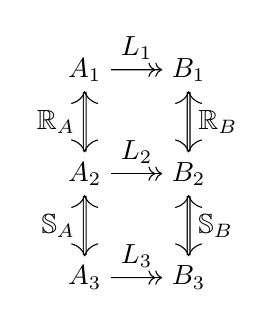
\begin{tikzpicture}[baseline,scale=0.66]
    \node (A1) at (-1,  2) {$A_1$};
    \node (A2) at (-1,  0) {$A_2$};
    \node (A3) at (-1, -2) {$A_3$};
    \node (B1) at ( 1,  2) {$B_1$};
    \node (B2) at ( 1,  0) {$B_2$};
    \node (B3) at ( 1, -2) {$B_3$};
    \draw (A1) edge[->>] node[auto] {$L_1$} (B1);
    \draw (A2) edge[->>] node[auto] {$L_2$} (B2);
    \draw (A3) edge[->>] node[auto] {$L_3$} (B3);
    \draw (A1) edge[<->, double] node[auto,swap] {$\mathbb{R}_A$} (A2);
    \draw (B1) edge[<->, double] node[auto] {$\mathbb{R}_B$} (B2);
    \draw (A2) edge[<->, double] node[auto,swap] {$\mathbb{S}_A$} (A3);
    \draw (B2) edge[<->, double] node[auto] {$\mathbb{S}_B$} (B3);
  \end{tikzpicture}
  $
  \caption{Simulation identity and composition}
  \label{fig:simcomp}
\end{figure}
%}}}

\paragraph{Simulation algebra} %{{{

We equip simulation conventions
with their own notion of refinement $\scref$,
which means a convention can replace another
in all simulation statements.
We can then construct a Kleene algebra
based on the composition and refinement of simulation conventions.

%}}}

\paragraph{Compiler correctness} \label{sec:compcert:overview} %{{{

These techniques allow us to formulate an overall
simulation convention
$\mathbb{C} : \mathcal{C} \Leftrightarrow \mathcal{A}$
for the compiler which is both compositional
and independent of the exact sequence of passes
included in the compiler.
We show that for a source program $p$
compiled to the target program $p'$,
the following simulation property holds:
\[
    \kw{Clight}(p)
    \le_{\mathbb{C} \twoheadrightarrow \mathbb{C}}
    \kw{Asm}(p') \,.
\]

%In Compositional CompCert,
%this is achieved independently for each compilation pass.
%Stated in our terms,
%Compositional CompCert
%employs a fixed interface $\mathcal{C}$,
%and \emph{structured injections} define a refinement convention
%$\mathbb{S} : \mathcal{C} \Leftrightarrow \mathcal{C}$.
%A theorem similar to (\ref{eqn:correctness}) is proved for each pass,
%and structured injections are shown to compose
%($\mathbb{S} \cdot \mathbb{S} \equiv \mathbb{S}$),
%so that a theorem can be derived for the whole compiler.

%A major challenge encountered in this context
%is the asymmetry of requirements vs. guarantees
%present in the existing proofs:
%while CompCert imposes strong requirements
%on the semantics of external functions,
%the simulation relations used by its correctness proofs
%are too weak to establish corresponding guarantees
%for a module's own function executions,
%preventing horizontal compositionality.
%Because of this,
%Compositional CompCert required significant changes
%to all compilation passes,
%strengthening their simulation relations
%to conform to $\mathbb{S}$.

%Our explicit treatment of abstraction
%and reified notion of simulation convention
%makes another approach possible.
%Existing proofs can be adapted to establish
%for each pass:
%\begin{equation}
%    \label{correctness-alt}
%    \llbracket p_t \rrbracket
%    \le_{\mathbb{R} \rightarrow \mathbb{R}'}
%    \llbracket p_s \rrbracket \,,
%\end{equation}
%where the simulation conventions $\mathbb{R}$ and $\mathbb{R}'$
%characterize the assumptions and guarantees of the proof.
%In addition,
%relevant properties of key source, target, and intermediate languages
%can be expressed in relational form,
%and can be used to strengthen the resulting theorem:
%by composing these proofs together,
%and using algebraic properties of
%the simulation conventions involved,
%we are able to bridge the gap
%between the domain and codomain simulation conventions
%and prove a correctness statement
%in the form of (\ref{eqn:correctness}),
%enabling horizontal compositionality.

%}}}

%}}}

\begin{table} % tbl:notations {{{
  \small
  \begin{tabular}{lcl}
    \hline
    Notation & Examples & Description \\
    \hline
    $R \in \mathcal{R}(S_1, S_2)$ &
      $\vref$ &
      Simple relation \\
    $R \in \mathcal{R}_W(S_1, S_2)$ &
      $\hookrightarrow_\kw{m}$ &
      Kripke relation (Def.~\ref{def:klr}) \\
    $w \Vdash R$ & &
      Kripke relation at world $w$ \\
    $w \Vdash x \mathrel{R} y$ & &
      $x$ and $y$ related at world $w$ \\
    \hline
    $A, B, C$ &
      $\mathcal{C}, \mathcal{A}, \mathbf{1}$ &
      Language interface (Def.~\ref{def:li}) \\
    %$M_A^\que, M_A^\ans$ & &
    %  Questions and answers of $A$ \\
    $L : A \twoheadrightarrow B$ &
      $\kw{Clight}(p)$ &
      LTS for $A \twoheadrightarrow B$ (Def.~\ref{def:lts}) \\
    $\mathbb{R} : A_1 \Leftrightarrow A_2$ &
      $\kw{alloc}, \mathbf{R}_\mathcal{C}$ &
      Simulation convention (Def.~\ref{def:simconv}) \\
    $L_1 \le_{\mathbb{R} \twoheadrightarrow \mathbb{S}} L_2$ &
      Thm.~\ref{thm:compc} &
      Simulation property (Def.~\ref{def:sim}) \\
    $L_1 \oplus L_2$ & &
      Horizontal composition (Def.~\ref{def:hcomp}) \\
    %$p_1 + p_2$ & &
    %  Program linking \\
    $\mathbf{R}$ &
      $\kw{ext}, \kw{inj}$ &
      CKLR (Def.~\ref{def:cklr}) \\
    \hline
  \end{tabular}
  \caption{Summary of notations}
  \label{tbl:notations}
\end{table}
%}}}

%}}}

\section{Operational semantics} \label{sec:sem} %{{{

%This section describes CompCertO's semantic infrastructure.
%In \S\ref{sec:sem:overview}--\ref{sec:sem:mm},
%we review the techniques used in CompCert
%to formalize the semantics of the various languages involved,
%then starting with \S\ref{sec:sem:open}
%we describe the extensions we use
%to model the behavior of \emph{open} programs.

\subsection{Overview} \label{sec:sem:overview} %{{{

The semantics of CompCert languages
are given in terms of a simple notion of process behavior.
By \emph{process}, we mean a self-contained computation
which can be characterized by
the sequence of system calls it performs.
%Several steps are involved to go
%from a source program to an executing process;
%these steps are modeled by CompCert
%with varying degrees of sophistication and accuracy.

For a C program to be executed,
its translation units must first be compiled to object code.
The object files are then linked together
into an executable binary.
Finally, the system loads the executable into memory
where bootstrap code sets up the process
and invokes the program's \texttt{main} function.

\begin{figure} % fig:process {{{
    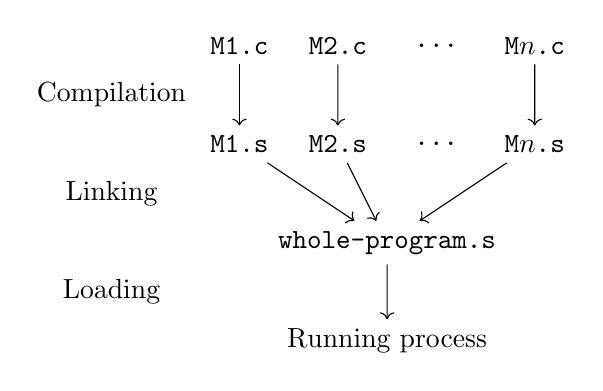
\begin{tikzpicture}[scale=1.25]
        \node (Mb) at (1.5, 0) {Running process};
        \tt
        \node (Ms) at (1.5, 1) {whole-program.s};
        \node (M1c) at (0, 3) {M1.c};
        \node (M2c) at (1, 3) {M2.c};
        \node (etc) at (2, 3) {\ldots};
        \node (Mnc) at (3, 3) {M$n$.c};
        \node (M1s) at (0, 2) {M1.s};
        \node (M2s) at (1, 2) {M2.s};
        \node (ets) at (2, 2) {\ldots};
        \node (Mns) at (3, 2) {M$n$.s};
        \draw (M1c) edge[->] (M1s);
        \draw (M2c) edge[->] (M2s);
        \draw (Mnc) edge[->] (Mns);
        \draw (M1s) edge[->] (Ms);
        \draw (M2s) edge[->] (Ms);
        \draw (Mns) edge[->] (Ms);
        \draw (Ms) edge[->] (Mb);
        \rm
        \node at (-1.3, 2.5) {Compilation};
        \node at (-1.3, 1.5) {Linking};
        \node at (-1.3, 0.5) {Loading};
        %\tt
        %\node (Mc) at (1.5, 4) {whole-program.c};
        %\draw (M1c) edge[->,dotted] (Mc);
        %\draw (M2c) edge[->,dotted] (Mc);
        %\draw (Mnc) edge[->,dotted] (Mc);
    \end{tikzpicture}
    \caption{CompCert's approximation of the C toolchain}
    \label{fig:process}
\end{figure}
%}}}

%Since CompCert is a compiler from C to assembly,
%but does not include an assembler or linker,
The model used for verifying CompCert accounts for
some of these aspects in the simplified way
depicted in Fig.~\ref{fig:process}.
%The lowest-level objects considered
%are CompCert \kw{Asm} programs.
Linking is approximated by
merging programs, seen as sets of global definitions.
The execution
of a program composed of the modules
$\texttt{M1.c} \ldots \texttt{M$n$.c}$
having respectively been compiled to
$\texttt{M1.s} \ldots \texttt{M$n$.s}$
is modeled as:
\[
    L_\kw{tgt} :=
    \kw{Asm}(\texttt{M1.s} +
             \cdots +
             \texttt{M$n$.s}) \,,
\]
where
$+$ denotes CompCert's linking operator and
$\kw{Asm}(-)$ maps an assembly program to its semantics.
Note that the loading process is encoded
as part of the definition of $\kw{Asm}$,
which constructs a global environment
laying out the program's code and static data
into the runtime address space,
and models the conventional invocation of \texttt{main}.

To formulate compiler correctness,
we must also specify the behavior of the source program.
To this end,
CompCert defines a linking operator
and semantics
for the language $\kw{Clight}$,%
\footnote{
  Although CompCert features a frontend for a richer version
  of the C language,
  the simplified intermediate dialect \kw{Clight}
  is usually used as the source language
  when using CompCert to build certified artifacts.
  In particular it is the target language of the
  \texttt{clightgen} utility which
  produces Coq code for a C program's AST,
  which the user can then prove to be correct
  either manually or with tools such as the VST program logic
  \cite{vst}.
}
allowing the desired behavior to be specified as:
\[
    L_\kw{src} :=
    \kw{Clight}(\texttt{M1.c} + \cdots + \texttt{Mn.c}) \,,
\]
and correctness of CompCert
%as a separate compiler
to be stated as $L_\kw{src} \sqsubseteq L_\kw{tgt}$.

%}}}

\subsection{Transition systems in CompCert} \label{sec:sem:closed} %{{{

In the original CompCert, language semantics are
given as labelled transition systems (LTS),
which characterize a program's behavior in terms of
sequences of observable events.

Schematically, a CompCert LTS
is a tuple
$L = \langle S, I, {\rightarrow}, F \rangle$
consisting of
a set of states $S$,
a subset $I \subseteq S$ of initial states,
a labelled transition relation
${\rightarrow} \subseteq S \times \mathbb{E}^* \times S$,
and a set
$F \subseteq S \times \kw{int}$
of final states associated with exit statuses.
The relation~$s \stackrel{t}{\rightarrow} s'$
indicates that the state $s$ may transition to the state $s'$
through an interaction $t \in \mathbb{E}^*$.
The possible behaviors of CompCert LTS fall into four categories:
\begin{itemize}
\item An execution reaching a final state is said to
    \emph{terminate}.
    For example,
    the following execution generates
    the event trace $t_1 t_2 \cdots t_{n-1}$
    and terminates with status $r$:
    \[
        I \ni s_1 \stackrel{t_1}{\rightarrow}
          s_2 \stackrel{t_2}{\rightarrow}
          \cdots \stackrel{t_{n-1}}{\rightarrow}
          s_n \mathrel{F} r \,.
    \]
\item An execution reaching
    an infinite sequence of $\epsilon$ transitions
    is said to \emph{silently diverge}.
    The following execution diverges after
    generating the trace $t_1 t_2 \cdots t_{n-1}$:
    \[
        I \ni s_1 \stackrel{t_1}{\rightarrow}
          s_2 \stackrel{t_2}{\rightarrow}
          \cdots \stackrel{t_{n-1}}{\rightarrow}
          s_n \stackrel{\epsilon}{\rightarrow}
          s_{n+1} \stackrel{\epsilon}{\rightarrow}
          \cdots
    \]
\item By contrast,
    infinite executions which keep interacting
    are said to exhibit \emph{reactive} behavior.
    The following execution
    is reactive if and only if
    $\forall i \, \exists j \,.\, i \le j \wedge t_j \ne \epsilon$:
    \[
        I \ni s_1 \stackrel{t_1}{\rightarrow}
          s_2 \stackrel{t_2}{\rightarrow}
          s_3 \stackrel{t_3}{\rightarrow}
          \cdots
    \]
\item Finally, an execution which reaches a stuck state
    is said to \emph{go wrong}. It will have the shape:
    \[
        I \ni s_1 \stackrel{t_1}{\rightarrow}
          s_2 \stackrel{t_2}{\rightarrow}
          \cdots \stackrel{t_{n-1}}{\rightarrow}
          s_n \,,
    \]
    with no $t, s'$ such that
    $s_n \stackrel{t}{\rightarrow} s'$.
    This models \emph{undefined behavior}
    and can be refined by any behavior
    admitting $t_1 t_2 \cdots t_{n-1}$ as a prefix.
\end{itemize}

%The model outlined above
%makes no attempt to model interactions across components,
%and is only ever used to
%describe the behavior of whole programs.
%This makes it challenging to reason about
%the behavior of individual compilation units,
%although there have been successful attempts in this direction
%\cite{sepcompcert,gilhurslatest}.
%In any case,
%the compiler's correctness property
%as described in \S\ref{sec:sem:intro}
%only considers uses which follow
%the pattern approximated in Fig.~\ref{fig:process}.
%
%To formulate a more fine-grained and flexible
%version of the correctness theorem of CompCert,
%we need an account of
%the behavior of individual translation units.
%The model presented in \S\ref{sec:sem:open}
%achives this by recoding control transfers
%to and from the modeled system explicitly.
%These control transfer will need to expose more information
%about the internal structure of program states;
%in the following section we review the design of
%CompCert's memory model,
%which all program states are constructed from.

The construction of states in CompCert language semantics
follow common patterns.
In particular,
all languages start with
the same notion of \emph{memory state}.

%}}}

\subsection{The CompCert memory model} \label{sec:sem:mm} %{{{

\begin{figure} % fig:mm (The CompCert memory model) {{{
  \begin{align*}
    v \in \kw{val} ::= {} &
          \kw{undef} \alt
          \kw{int}(n) \alt
          \kw{long}(n) \alt \\ &
          \kw{float}(x) \alt
          \kw{single}(x) \alt
          \kw{vptr}(b, o)
  \end{align*}
  \begin{align*}
    (b, o) &\in \kw{ptr} =
      \kw{block} \times \mathbb{Z}
    \\
    (b, l, h) &\in \kw{ptrrange} =
      \kw{block} \times \mathbb{Z} \times \mathbb{Z}
  \end{align*}
  \begin{align*}
    \kw{alloc} &:
      \kw{mem} \rightarrow \mathbb{Z} \rightarrow \mathbb{Z} \rightarrow
      \kw{mem} \times \kw{block}
    \\
    \kw{free} &:
      \kw{mem} \rightarrow
      \kw{ptrrange} \rightarrow
      \kw{option}(\kw{mem})
    \\
    \kw{load} &:
      \kw{mem} \rightarrow \kw{ptr} \rightarrow \kw{option}(\kw{val})
    \\
    \kw{store} &:
      \kw{mem} \rightarrow \kw{ptr} \rightarrow \kw{val} \rightarrow \kw{option}(\kw{mem})
    \\
    \kw{perm} &:
      \kw{mem} \rightarrow \kw{ptr} \rightarrow \mathcal{P}(\kw{perm})
  \end{align*}
  \caption{Outline of the CompCert memory model}
  \label{fig:mm}
\end{figure}
%}}}

The CompCert memory model \cite{compcertmm,compcertmmv2}
is the core algebraic structure
underlying the semantics of CompCert's languages.
Some of its operations
are shown in Fig.~\ref{fig:mm}.
The idealized version presented here
involves
the type of memory states \kw{mem},
the type of runtime values \kw{val}, and
the types of pointers \kw{ptr} and address ranges \kw{ptrrange}.
To keep our exposition concise and clear,
we gloss over the technical details
associated with modular arithmetic and overflow constraints.

The memory is organized into a finite number of \emph{blocks}.
Each memory block has a unique identifier $b \in \kw{block}$
%represented as a positive integer,
and is equipped with its own linear address space.
Block identifiers and offsets are often manipulated together
as pointers $p = (b, o) \in \kw{ptr} = \kw{block} \times \mathbb{Z}$.
New blocks are created with prescribed boundaries
using the primitive $\kw{alloc}$.

A runtime value $v \in \kw{val}$ can be stored at
a given address using the primitive \kw{store},
and retreived using the primitive \kw{load}.
Values can be integers (\kw{int}, \kw{long}) and
floating point numbers (\kw{float}, \kw{single})
of different sizes,
as well as pointers (\kw{vptr}).
The special value \kw{undef}
represents an undefined value;
simulation relations
often allow $\kw{undef}$
to be refined into a more concrete value.
We write value refinement as:
\[
    {\vref} := \{(\kw{undef}, v), (v, v) \mid v \in \kw{val}\} \,.
\]

The memory model is shared by all of the languages in CompCert.
States always consist of
a memory component $m \in \kw{mem}$,
alongside language-specific components
which may contain additional values ($\kw{val}$).

%}}}

\subsection{CompCertO's open semantics} \label{sec:sem:open} %{{{

The memory model also plays a central role
when describing interactions between program modules.
Under our approach to module semantics,
the memory state is passed back-and-forth
alongside all control transfers.

\paragraph{Language interfaces} %{{{

Our models of cross-module interactions in CompCert languages
are shown in Table~\ref{tbl:li}.
We call each one a \emph{language interface}.
Questions correspond to function invocations
and answers return control to the caller.
Formally,
a language interface is defined as follows.

\begin{definition} \label{def:li}
A \emph{language interface} is a tuple
$A = \langle M_A^\que, M_A^\ans \rangle$, where
$M_A^\que$ is a set of \emph{questions} and
$M_A^\ans$ is a set of \emph{answers}.
\end{definition}

At the source level ($\mathcal{C}$),
questions consist of
the address of the invoked function
($\mathit{vf} \in \kw{val}$),
its signature
($\mathit{sg} \in \kw{signature}$),
the values of its arguments
($\vec{v} \in \kw{val}^*$),
and the state of the memory at the point of entry
($m \in \kw{mem}$);
answers
consist of the function's return value
and the state of the memory at the point of exit.
In these terms,
a Clight component describes a strategy for the game
$\mathcal{C} \twoheadrightarrow \mathcal{C}$.
The component is activated by an incoming $\mathcal{C}$ question
in the right-hand side game,
where it is expected to produce a $\mathcal{C}$ answer.
In the meantime,
it may perform external calls by
asking questions and expecting answers
in the left-hand side $\mathcal{C}$ game.

This language interface is used for \kw{Clight} and
for the majority of CompCert's intermediate languages,
including \kw{RTL} which is used to perform
most of the compiler's optimizations.
As we move towards lower-level languages,
this is reflected in the language interfaces used:
function arguments are first mapped into
abstract locations alongside local temporary variables
($\mathcal{L}$, used by \kw{LTL} and \kw{Linear}).
These locations are eventually split between
in-memory stack slots and a fixed number of machine registers
($\mathcal{M}$, used by \kw{Mach}).
Finally, the target assembly language \kw{Asm}
stores the stack pointer, program counter,
and return address into their own machine registers,
which is reflected in its interface $\mathcal{A}$.

The interface of whole-program execution
can also be described in this setting:
the language interface $\mathbf{1}$ contains no move;
the interface $\mathcal{W}$ has a single trivial question $*$,
and the answers $r \in \kw{int}$
give the exit status of a process.
Hence the original CompCert semantics described in
\S\ref{sec:sem:closed}
can be seen to define strategies for
$\mathbf{1} \twoheadrightarrow \mathcal{W}$:
the process can only be started in a single way,
may not perform external calls,
and indicates an exit status upon termination.

%}}}

\begin{table} % tbl:li Language interfaces {{{
  \begin{tabular}{clll}
    \hline
    Name & Question & Answer & Description \\
    \hline
    $\mathcal{C}$ &
      $\mathit{vf}[\mathit{sg}](\vec{v})@m$ & $v'@m'$ &
      C calls \\
    $\mathcal{L}$ &
      $\mathit{vf}[\mathit{sg}](\mathit{ls})@m$ & $\mathit{ls}'@m'$ &
      Abstract locations \\
    $\mathcal{M}$ &
      $\mathit{vf}(\mathit{sp},\mathit{ra},\mathit{rs})@m$ & $\mathit{rs}'@m'$ &
      Machine registers \\
    $\mathcal{A}$ &
      $\mathit{rs}@m$ & $\mathit{rs}'@m'$ &
      Arch-specific \\
    $\mathbf{1}$ & n/a & n/a &
      Empty interface \\
    $\mathcal{W}$ & * & $r$ &
      Whole-program \\
    \hline
  \end{tabular}
  \caption{Language interfaces used in CompCertO}
  \label{tbl:li}
\end{table}
%}}}

\paragraph{Transition systems} %{{{

CompCertO generalizes
the semantic model of
\S\ref{sec:sem:closed}
to account for cross-component interactions.

\begin{definition} \label{def:lts}
Given an \emph{incoming} language interface $B$
and an \emph{outgoing} language interface $A$,
a \emph{labelled transition system for the game $A \twoheadrightarrow B$}
is a tuple $L = \langle S, \rightarrow, D, I, X, Y, F \rangle$.
The relation
${\rightarrow} \subseteq S \times \mathbb{E}^* \times S$ is
a \emph{transition relation} on the set of states $S$.
The set $D \subseteq M_B^\que$ specifies which
questions the component accepts;
$I \subseteq D \times S$ then
assigns to each one a set of \emph{initial states}.
$F \subseteq S \times M_B^\ans$,
designates \emph{final states} together with corresponding answers.
External calls are specified by
$X \subseteq S \times M_A^\que$,
which designates \emph{interacting states} together with
a question of $A$, and
$Y \subseteq S \times M_A^\ans \times S$,
which is used to select a \emph{resumption state}
to follow an interacting state
based on the answer provided by the environment.
We write $L : A \twoheadrightarrow B$ when
$L$ is a labelled transition system for $A \twoheadrightarrow B$.
\end{definition}

The interpretation of the generalized LTS described above
follows the one given in \S\ref{sec:sem:closed},
with interactions over the game $A$
as a new source of observable actions.
The main reason for treating
events $e \in \mathbb{E}$ and
external calls $m n \in M_A^\que \times M_A^\ans$
differently is that
while events are expected to be the same
between the source and target programs,
the form of external calls varies significantly
across languages
and the simulation convention they follow
must be defined explicitly.

%For a small-step semantics
%$L = \langle S, {\rightarrow}, I, X, Y, F \rangle : \kw{semantics}(A,B)$,
%we recognize those states using the predicate:
%\[
%    \kw{stuck}_L(s) :=
%      ({\rightarrow}(s) = \varnothing) \wedge
%      (X(s) = \varnothing) \wedge
%      (F(s) = \varnothing)
%\]
%Taking this into account,
%the immediate behavior of a state $s \in S$
%can be expressed as the interactive computation
%$\kw{step}_L(s) : \mathcal{I}_{M_A^\que,M_A^\ans}(S)$
%defined as follows:
%\[
%  \kw{step}_L(s) :=
%    \begin{cases}
%      \top & \mbox{if } \kw{stuck}(s) \\
%      {\rightarrow}(s) \sqcup
%      (X(s) \bind \mathbf{I} \bind Y(s)) & \mbox{otherwise,}
%   \end{cases}
%\]
%The overall external behavior of $L$
%can then be given as
%$
%    \llbracket L \rrbracket :
%      M_B^\que \rightarrow \mathcal{I}_{M_A^\que,M_A^\ans}(M_B^\ans)
%$
%defined by:
%%Then $\llbracket L \rrbracket$ can be defined as:
%\begin{align*}
%  \llbracket L \rrbracket (q) :=
%    \begin{cases}
%       \top & \mbox{if } I(q) = \varnothing \\
%       I(q) \bind \kw{step}^\infty \bind F & \mbox{otherwise.}
%     \end{cases}
%\end{align*}

%}}}

%}}}

\subsection{Forward simulations} \label{sec:sem:ref} %{{{

CompCert is proved correct using a simulation
between the transition semantics of the source and target programs.
This \emph{forward}%
\footnote{In this usage, \emph{forward} pertains to
  the compilation process,
  rather than the execution of programs.}
simulation is used to prove a \emph{backward} simulation.
Backward simulations
are in turn proved to be sound with respect to trace containement.
We have updated forward and backward simulations to
work with CompCertO's semantic model.
In this section we present forward simulations,
which will be used as our preferred notion of refinement.
%in the remainder of the paper.

To establish the correctness of the compiler
in terms of our per-module semantics,
we need to relate the behavior of the source component
$\kw{Clight}(p_1) : \mathcal{C} \twoheadrightarrow \mathcal{C}$,
and the behavior of the target program
$\kw{Asm}(p_2) : \mathcal{A} \twoheadrightarrow \mathcal{A}$.
Since these two LTS
use different language interfaces,
they can only be compared once a correspondance between
C and assembly calls has been defined.
This is the role of simulation conventions.

\begin{definition} \label{def:simconv} % Simulation convention %{{{
A \emph{simulation convention} between the language interfaces
$A_1 = \langle M_{A_1}^\que, M_{A_1}^\ans \rangle$ and
$A_2 = \langle M_{A_2}^\que, M_{A_2}^\ans \rangle$
is as a tuple $\mathbb{R} = \langle W, \mathbb{R}^\que, \mathbb{R}^\ans \rangle$
with $\mathbb{R}^\que \in \mathcal{R}_W(M_{A_1}^\que, M_{A_2}^\que)$
and $\mathbb{R}^\ans \in \mathcal{R}_W(M_{A_1}^\ans, M_{A_2}^\ans)$.
We will write $\mathbb{R} : A_1 \Leftrightarrow A_2$.
\end{definition}
%}}}

\begin{definition} % Identity simulation convention {{{
The \emph{identity simulation convention} for
a language interface $A$ is
$\kw{id}_A := \langle \{*\}, {=}, {=} \rangle : A \Leftrightarrow A$.
We abbreviate it as $\kw{id}$ when $A$ can be deduced
from context.
\end{definition}
%}}}

%The set of worlds $W$ is used to
%make sure that questions on one hand,
%and answers on the other hand,
%are related consistently.
%For instance,
%in CompCertO's overall simulation convention
%$\mathbb{C} : \mathcal{C} \Leftrightarrow \mathcal{A}$,
%the registers used to store a function's return value
%may depend on the signature $\kw{sg}$ used for the call.
%As another example,
%when an injection pass makes an external call,
%we need to make sure the call's final memory states
%are related by the same memory injection that was used
%for the initial states (or a successor, see \S\ref{sec:corr:inj}).

A forward simulation asserts that any transition in the source program
has a corresponding transition sequence in the target.
The sequence may be empty,
but to ensure the preservation of silent divergence
this can only happen for finitely many consecutive source transitions.
This is enforced by indexing the simulation relation
over a well-founded order,
and requiring the index to decrease
whenever an empty transition sequence is used.

%A simulation between the small-step semantics
%$L_1 : A_1 \rightarrow B_1$ and
%$L_2 : A_2 \rightarrow B_2$ will
%operate in the context of the refinement conventions
%$\mathbb{C}_A : A_1 \Leftrightarrow A_2$ and
%$\mathbb{C}_B : B_1 \Leftrightarrow B_2$.
%When relating sets of states,
%we will want to make sure that
%each \emph{target} state has a corresponding \emph{source} state,
%but the source program may allow additional behaviors
%that are not realized in the target program.
%However, to take into account the convention that
%empty sets of states correspond to undefined behaviors,
%when the source set is empty,
%no restrictions are placed on the target state.
%
%\begin{definition}[Backward simulation between sets of states]
%We say that $R : \mathcal{R}(S_1, S_2)$ is a
%\emph{backward simulation relation
%  between the sets $Q_1 \subseteq S_1$ and  $Q_2 \subseteq S_2$}
%if the following conditions hold:
%\begin{enumerate}
%\item
%  If $Q_1$ is non-empty,
%  then $Q_2$ is non-empty as well.
%\item
%  If $Q_1$ is non-empty,
%  then for all $s_2 \in Q_2$,
%  there exists $s_1 \in Q_1$
%  such that $(s_1, s_2) \in R$.
%\end{enumerate}
%We will write $Q_1 \ge_R Q_2$.
%\end{definition}
%
%A state $s$ \emph{goes wrong}
%if it is neither an interaction nor a final state,
%and if there is no transition $s \stackrel{t}{\rightarrow} s'$;
%a state $s$ is \emph{safe}
%if no state that goes wrong is reachable from $s$
%by the relation $\stackrel{\epsilon}{\rightarrow}$.
%Safe states will be denoted using the predicate $\kw{safe}(s)$.
%We can now define backward simulations.

\begin{definition}[Forward simulation] \label{def:sim}
Given
two simulation conventions
$\mathbb{R}_A : A_1 \Leftrightarrow A_2$ and
$\mathbb{R}_B : B_1 \Leftrightarrow B_2$,
and given
the transition systems
$L_1 : A_1 \twoheadrightarrow B_1$ and
$L_2 : A_2 \twoheadrightarrow B_2$,
a \emph{forward simulation} between $L_1$ and $L_2$
consists of a
well-founded relation $(I, <)$
together with a family of relations
$(R_i : \mathcal{R}_{W_B}(S_1, S_2))_{i \in I}$
satisfying the following properties:
\begin{description}
\item[Domains]
  For all
  $w_B \Vdash q_1 \mathrel{\mathbb{R}_B^\que} q_2, \:\:
   q_1 \in D_1 \Leftrightarrow q_2 \in D_2$.
\item[Initial states]
  For
  $w_B \Vdash q_1 \mathrel{\mathbb{R}_B^\que} q_2$
  with $q_1 \mathrel{I_1} s_1$,
  there exist $i \in I, s_2 \in S_2$
  such that $q_2 \mathrel{I_2} s_2$ and
  $w_B \Vdash s_1 \mathrel{R_i} s_2$.
\item[Simulation]
  For $w_B \Vdash s_1 \mathrel{R_i} s_2$
  with $s_1 \stackrel{t}{\rightarrow} s_1'$,
  there exist $i' \in I$ and $s_2' \in S_2$
  such that $w_B \Vdash s_1' \mathrel{R_{i'}} s_2'$ and
  such that
    $s_2 \mathrel{\stackrel{t}{\rightarrow}{\!\!}^+} s_2'$ or
    $s_2 \mathrel{\stackrel{t}{\rightarrow}{\!\!}^*} s_2' \:\wedge\: i' < i$.
\item[External calls]
  For $w_B \Vdash s_1 \mathrel{R_i} s_2$
  with $s_1 \mathrel{X_1} m_1$,
  there exist $w_A \in W_A$ and $m_2 \in M_{A_2}^\que$
  with $w_A \Vdash m_1 \mathrel{\mathbb{R}_A^\que} m_2$,
  such that for all
  $w_A \Vdash n_1 \mathrel{\mathbb{R}_A^\ans} n_2$
  and $s_1' \in S_1$ with $(s_1, n_1, s_1') \in Y_1$,
  there exists $s_2' \in S_2$ st.
  $(s_2, n_2, s_2') \in Y_2$.
\item[Final states]
  For $w_B \Vdash s_1 \mathrel{R_i} s_2$
  with $s_1 \mathrel{F_1} r_1$,
  there exists $r_2 \in M_{B_2}^\ans$ such that
  $s_2 \mathrel{F_2} r_2$ and $w_B \Vdash r_1 \mathrel{\mathbb{R}_B^\ans} r_2$.
\end{description}
We will write $L_1 \le_{\mathbb{R}_A \twoheadrightarrow \mathbb{R}_B} L_2$.
\end{definition}

%}}}

\subsection{Horizontal composition} \label{sec:sem:linker} %{{{

The interaction of a set of components
can be modelled by the following operator.

\begin{definition}[Horizontal composition] \label{def:hcomp} %{{{
For two transition systems $L_1, L_2 : A \rightarrow A$
with
$L_i = \langle S_i, {\rightarrow}_i, D_i, I_i, X_i, Y_i, F_i \rangle$,
the \emph{horizontal composition} of $L_1$ and $L_2$
is defined as:
\[
    L_1 \oplus L_2 :=
    \langle
      (S_1 + S_2)^*, {\rightarrow}, D_1 \cup D_2, I, X, Y, F
    \rangle
\]
where the components $\rightarrow$, $I$, $X$, $Y$, $F$
are defined inductively by
the rules shown in Fig.~\ref{fig:hcomp}.
\end{definition}
%}}}

\begin{figure} % fig:hcomp {{{
    \footnotesize
    \begin{gather*}
        \AxiomC{$q \in D_i$}
        \AxiomC{$q \mathrel{I_i} s$}
        \BinaryInfC{$q \mathrel{I} [(i, s) :: \kw{nil}]$}
        \DisplayProof
        \quad
        \AxiomC{$s \stackrel{t}{\rightarrow}_i s'$}
        \UnaryInfC{$
            [(i, s) :: k]
            \stackrel{t}{\rightarrow}
            [(i, s') :: k]$}
        \DisplayProof
        \quad
        \AxiomC{$s \mathrel{F_i} r$}
        \UnaryInfC{$[(i, s) :: \kw{nil}] \mathrel{F} r$}
        \DisplayProof
        \\[1ex]
        \AxiomC{$s \mathrel{X_i} q$}
        \AxiomC{$q \in D_j$}
        \AxiomC{$q \mathrel{I_j} s'$}
        \TrinaryInfC{$
            [(i, s) :: k]
            \stackrel{\epsilon}{\rightarrow}
            [(j, s') :: (i, s) :: k]$}
        \DisplayProof
        \quad
        \AxiomC{$s' \mathrel{F_j} r$}
        \AxiomC{$(s, r, s'') \in Y_i$}
        \BinaryInfC{$
            [(j, s') :: (i, s) :: k]
            \stackrel{\epsilon}{\rightarrow}
            [(i, s'') :: k]$}
        \DisplayProof
        \\[1ex]
        \AxiomC{$s \mathrel{X_i} q$}
        \AxiomC{$\forall j \,.\, q \notin D_j$}
        \BinaryInfC{$[(i, s) :: k] \mathrel{X} q$}
        \DisplayProof
        \qquad
        \AxiomC{$(s, r, s') \in Y_i$}
        \UnaryInfC{$([(i, s) :: k], r, [(i, s') :: k]) \in Y$}
        \DisplayProof
    \end{gather*}
    \caption{Horizontal composition of open semantics}
    \label{fig:hcomp}
\end{figure}
%}}}

The definition above
assumes that the components are determinate,
which is indeed the case for the range of languages
we are interested in.
It keeps track of a stack of alternating activations
of the two components.
During normal execution,
only the top-level state is updated.
External calls to functions which are provided by the other component
are handled by pushing a new state of that component onto the stack,
initialized by the call in question.
If a final state is reached
while there are suspended activations,
we use the result to resume the most recent one.
External calls which are provided by neither component,
and final states encountered at the top level,
are simply passed along to the environment.

The horizontal composition operator
allows us to decompose the verification of a complex program
into the verification of its parts.
Since we want to
establish the correctness of assembly programs,
the following theorem showing the correctness
of assembly linking is particularly critical.

\begin{theorem} \label{thm:asmlinking} %{{{
For \kw{Asm} programs,
linking is a correct implementation of
horizontal composition:
\[
    \forall p_1 p_2 \,.\,
      \kw{Asm}(p_1) \oplus \kw{Asm}(p_2)
      \le_\kw{id}
      \kw{Asm}(p_1 + p_2)
\]
\begin{proof}
See \texttt{x86/AsmLinking.v} in the Coq development.
\end{proof}
\end{theorem}
%}}}

Once the semantics of the \kw{Asm} program
has been split into its components,
we can verify each one independently.
This is enabled by the following property.
%namely the preservation of simulations by
%horizontal composition.

\begin{theorem} \label{thm:simlinking} %{{{
For a simulation convention
$\mathbb{R} : A_1 \Leftrightarrow A_2$
and transition systems
$L_1, L_1' : A_1 \rightarrow A_1$ and
$L_2, L_2' : A_2 \rightarrow A_2$,
the following propery holds:
\[
    \AxiomC{$L_1 \le_{\mathbb{R} \rightarrow \mathbb{R}} L_2$}
    \AxiomC{$L_1' \le_{\mathbb{R} \rightarrow \mathbb{R}} L_2'$}
    \BinaryInfC{$L_1 \oplus L_1' \le_{\mathbb{R} \rightarrow \mathbb{R}} L_2 \oplus L_2'$}
    \DisplayProof
\]
\begin{proof}
See \texttt{common/SmallstepLinking.v}
in the Coq development,
specifically \texttt{compose\_simulation}.
\end{proof}
\end{theorem}
%}}}

%}}}

%\subsection{Loaders} \label{sec:sem:loader} %{{{
%
%XXX: Here, could describe how loaders for various language
%interfaces can be defined.
%Loaders turn an open semantics such as
%$L : \mathcal{C} \rightarrow \mathcal{C}$
%into a closed whole-program semantics of type
%$\kw{load}(L) : \mathbf{1} \rightarrow \mathcal{W}$.
%
%Problem: the definitions of loaders involve
%program skeletons and symbol tables,
%which so far I have left out of the semantic model.
%
%}}}

%}}}

\section{Logical relations for CompCert} \label{sec:cklr} %{{{

Language interfaces reveal the information
associated with function calls and returns
at different levels of abstraction.
Simulation conventions
reveal corresponding aspects of the simulation relations
used in CompCert's proofs.
%
The states of CompCert languages all contain
a memory state and surrounding runtime values.
Likewise, simulation relations
are constructed around \emph{memory transformations}
and relate the surrounding components in ways that %,
%in addition to reflecting any structural changes
%between to source and target language interfaces,
are compatible with the chosen memory transformation.

\subsection{Memory extensions} \label{sec:memext} %{{{

For passes where strict equality is too restrictive,
but the source and target programs
use similar memory layouts,
CompCert uses the \emph{memory extension} relation,
which allows the values
stored in the target memory state to refine
the values stored in the source memory at the same location.
%the target memory state can also
%provide more permissions than the source memory,
%and in particular blocks may be allocated with
%a broader range of addresses in the target memory
%than in the source memory.

We write $m_1 \mext m_2$ to signify that
the source memory $m_1$ is extended by
the target memory $m_2$,
by analogy with
the value refinement relation $v_1 \vref v_2$
introduced in $\S\ref{sec:sem:mm}$.
Together,
they
constitute a logical relation for the memory model,
in the sense that
loads from memory states related by extension
yield values related by refinement,
writing values related by refinement
preserves memory extension,
and similarly for the remaining memory operations.

%}}}

\subsection{Memory injections} \label{sec:meminj} %{{{

The most complex simulation relations of CompCert
allow memory blocks to be dropped, added, or
mapped at a given offset within a larger block.
These transformations of the memory structure
are specified by partial functions of type:
\[
  \kw{meminj} := \kw{block} \rightharpoonup \kw{block} \times \mathbb{Z} \,,
\]
We will call $f \in \kw{meminj}$
an \emph{injection mapping}.
An entry $f(b) = (b', o)$
means that the source memory block with identifier $b$
is mapped into the target block $b'$
at offset $o$.

As with refinement and extension,
an injection mapping determines both
a relation on values and
a relation on memory states,
which work together
as a logical relation for the CompCert memory model.
The relation $f \Vdash v_1 \hookrightarrow_\kw{v} v_2$
allows $v_2$ to refine $v_1$,
but also requires any pointer present in $v_1$ 
to be transformed according to $f$.
The relation $f \Vdash m_1 \hookrightarrow_\kw{m} m_2$
requires that the corresponding addresses of $m_1$ and $m_2$
hold values that are related by $f \Vdash {\hookrightarrow_\kw{v}}$.
%The injection mapping $f$ plays the role of a Kripke world,
%ensuring that the memory states and surrounding values
%are related consistently.

Note that corresponding memory allocations
in the source and target states cause $f$ to
evolve into a more defined injection mapping $f \subseteq f'$
relating the two newly allocated blocks.
To handle this,
we introduce the following constructions.

%}}}

\subsection{Modal Kripke relators} %{{{

We defined general Kripke relations in \S\ref{sec:logrel}.
We add structure to sets of Kripke worlds,
specifying how they can evolve.

\begin{definition} %{{{
A \emph{Kripke frame} is a tuple
$\langle W, {\leadsto} \rangle$, where
$W$ is a set of \emph{possible worlds} and
$\leadsto$ is a
binary \emph{accessibility relation} over $W$.
Then the Kripke relator $\Diamond$ is defined by:
\[
  w \Vdash x \ifr{\Diamond R} y \: \Leftrightarrow \:
    \exists \, w' \,.\, w \leadsto w' \wedge
      w' \Vdash x \mathrel{R} y
\]
\end{definition}
%}}}

\begin{example}[Injection simulation diagrams] \label{ex:sim} %{{{
Consider the simple transition systems
$\alpha : A \rightarrow \mathcal{P}(A)$ and
$\beta : B \rightarrow \mathcal{P}(B)$.
An injection-based simulation relation between them
will be a Kripke relation
$R \in \mathcal{R}_\kw{meminj}(A, B)$
satisfying the property:
\[
  \begin{tikzcd}
    s_1 \arrow[r, "\alpha"]
        \arrow[d, dash, "R_f"'] &
    s_1' \arrow[d, dashed, dash, "R_{f'} \quad (f \subseteq f')"] \\
    s_2 \arrow[r, dashed, "\beta"] &
    s_2'
  \end{tikzcd}
\]
More precisely, this diagram represents the condition:
\begin{equation}
    \label{eqn:hairy-sim}
    \begin{array}{r@{}l}
    \forall f \, s_1 \, s_2 \, s_1' \,.\,
      f \Vdash s_1 \mathrel{R} s_2 &{} \wedge
      \alpha(s_1) \ni s_1' \Rightarrow \\
    \exists f' \, s_2' \,.\,
      f \subseteq f' &{} \wedge
      \beta(s_2) \ni s_2' \wedge
      f' \Vdash s_1' \mathrel{R} s_2'
    \end{array}
\end{equation}
Here, the new states may be related according to
a new injection mapping $f'$,
but in order to preserve existing relationships
between any surrounding source and target pointers,
the new mapping should include
the original one ($f \subseteq f'$).

This pattern is very common in CompCert
and appears in a variety of contexts.
By using $\langle \kw{meminj}, {\subseteq} \rangle$
as a Kripke frame,
we can express it concisely and compositionally
in our relational framework.
For instance,
using the relator $\mathcal{P}^\le$ defined in
Fig.~\ref{fig:relators},
the condition (\ref{eqn:hairy-sim}) above can be expressed
as:
\[
  \alpha \ifr{\Vdash R \rightarrow \mathcal{P}^\le(\Diamond R)} \beta \,.
\]
\end{example}
%}}}

%}}}

\subsection{CompCert Kripke logical relations} \label{sec:cklrdef} %{{{

We can now formalize the idea that
extensions and injections
constitute logical relations for the CompCert memory model.

\begin{definition}[CompCert Kripke Logical Relation] \label{def:cklr} %{{{
For a tuple $R = (W, \leadsto, f, R^\kw{mem})$,
where
$\langle W, \leadsto \rangle$ is a Kripke frame,
$f : W \rightarrow \kw{meminj}$
associates an injection mapping to each world, and where
$R^\kw{mem} \in \mathcal{R}_{W}(\kw{mem})$
is a Kripke relation on memory states,
the Kripke relations
$R^\kw{ptr} \in \mathcal{R}_W(\kw{ptr})$ and
$R^\kw{ptrrange} \in \mathcal{R}_W(\kw{ptrrange})$
are defined by the rules:
\begin{gather*}
  \AxiomC{$f_w(b) = (b', \delta)$}
  \UnaryInfC{$w \Vdash (b, o) \mathrel{R^\kw{ptr}} (b', o + \delta)$}
  \DisplayProof
  \\[1ex]
  \AxiomC{$w \Vdash (b_1, l_1) \mathrel{R^\kw{ptr}} (b_2, l_2)$}
  \AxiomC{$h_1 - l_1 = h_2 - l_2$}
  \BinaryInfC{$w \Vdash (b_1, l_1, h_1) \mathrel{R^\kw{ptrrange}} (b_2, l_2, h_2)$}
  \DisplayProof
\end{gather*}
and
$R^\kw{val} \in \mathcal{R}_W(\kw{val})$
is the smallest Kripke relation satisfying:
\begin{gather*}
  \forall \, v \in \kw{val} \,.\,
    \Vdash \kw{undef} \mathrel{R^\kw{val}} v \qquad
  \kw{vptr} :: {\Vdash R^\kw{ptr} \rightarrow R^\kw{val}} \\
  \kw{int}, \kw{long}, \kw{float}, \kw{single} ::
    {\Vdash {=} \rightarrow R^\kw{val}} \,.
\end{gather*}
We say that $R$ is a \emph{CompCert Kripke logical relation}
if the properties shown in Fig.~\ref{fig:cklr-def} are satisfied.
\end{definition}
%}}}

\begin{figure} % fig:cklr-def (Definition of CKLRs) {{{
  \begin{gather*}
    {\leadsto} \mbox{ is reflexive and transitive} \\
    w \leadsto w' \Rightarrow f(w) \subseteq f(w')
  \end{gather*}
  \begin{align*}
      \kw{alloc} ::
        &\Vdash R^\kw{mem} \rightarrow {=} \rightarrow {=} \rightarrow
        \Diamond (R^\kw{mem} \times R^\kw{block})
      \\
      \kw{free} ::
        &\Vdash R^\kw{mem} \rightarrow R^\kw{ptrrange} \rightarrow
        \kw{option}^\le(\Diamond R^\kw{mem})
      \\
      \kw{load} ::
        &\Vdash R^\kw{mem} \rightarrow R^\kw{ptr} \rightarrow
        \kw{option}^\le(R^\kw{val})
      \\
      \kw{store} ::
        &\Vdash R^\kw{mem} \rightarrow R^\kw{ptr} \rightarrow R^\kw{val} \rightarrow
        \kw{option}^\le(\Diamond R^\kw{mem})
      \\
      \kw{perm} ::
        &\Vdash R^\kw{mem} \rightarrow R^\kw{ptr} \rightarrow {\subseteq}
  \end{align*}
  \caption{Defining properties of CKLRs}
  \label{fig:cklr-def}
\end{figure}
%}}}

We expect $R^\kw{ptr}$ to map
each source pointer to at most one target pointer,
and to satisfy the shift-invariance property:
\[
  \AxiomC{$w \Vdash (b_1, o_1) \mathrel{R^\kw{ptr}} (b_2, o_2)$}
  \UnaryInfC{$w \Vdash (b_1, o_1 + \delta) \mathrel{R^\kw{ptr}} (b_2, o_2 + \delta)$}
  \DisplayProof
\]
Any such relation can be uniquely specified by
the injection mapping $f$.
The relation $R^\kw{mem}$ is given.
We expect the other relations to be consistent with $R^\kw{ptr}$
and $\kw{undef}$ to act as a least element for $R^\kw{val}$,
which determines them completely.
Furthermore, owing to the relational property associated with $f$,
the derived relations are monotonic in $w$.
This may not be the case for $R^\kw{mem}$,
which is the central component driving world transitions,
as witnessed by the uses of $\Diamond$ in Fig.~\ref{fig:cklr-def}.
But this means that any surrounding state
constructed from pointers and runtime values
will be able to ``follow along'' when
world transitions do occur.

\begin{theorem}
The following definitions capture extensions and
injections as CompCert Kripke logical relations:
\begin{align*}
  \kw{ext} &:=
    \langle \{*\}, \: \{(*,*)\}, \: * \mapsto (b \mapsto (b, 0)), \:
    {\mext} \rangle
  \\
  \kw{inj} &:=
    \langle \kw{meminj}, {\subseteq}, f \mapsto f,
      {\hookrightarrow_\kw{m}} \rangle
\end{align*}
\begin{proof}
The correspondance between $R^\kw{val}_\kw{inj}$ and
$\hookrightarrow_\kw{v}$ is easily verified,
as is the correspondance between
$* \Vdash R^\kw{val}_\kw{ext}$ and $\vref$.
The properties of Fig.~\ref{fig:cklr-def}
reduce to well-known properties of the memory model
already proven in CompCert.
See \texttt{cklr/Extends.v} and \texttt{cklr/Inject.v}
for details.
\end{proof}
\end{theorem}

%}}}

\subsection{From CKLRs to simulation conventions} \label{sec:param} %{{{

Given a specific language interface $\mathcal{X}$,
the components of any CKLR
$R = \langle W, {\leadsto}, f, R^\kw{mem} \rangle$
can be used to construct a simulation relation
$R_\mathcal{X} : \mathcal{X} \Leftrightarrow \mathcal{X}$.
For instance:
\[
  R_\mathcal{C} :=
    \langle
      W, \:
      (R^\kw{val} \times {=} \times \vec{R}^\kw{val} \times R^\kw{mem}), \:
      \Diamond (R^\kw{val} \times R^\kw{mem})
    \rangle \,.
\]
We will omit the subscript $\mathcal{C}$ when we know from context
that a certain kind of simulation convention is needed.

Furthermore,
since the semantics of CompCert languages
are built out of the operations of the memory model,
they are well-behaved with respect to CKLRs and
we can prove the following parametricity theorems.

\begin{theorem}[Relational parametricity of $\kw{Clight}$ and $\kw{RTL}$] %{{{
\label{thm:param}
The following properties hold for all programs:
\begin{gather*}
    \forall R \,.\,
      \kw{Clight}(p)
        \le_{R_\mathcal{C} \twoheadrightarrow R_\mathcal{C}}
      \kw{Clight}(p)
      \label{eqn:clight}
      \\
    \forall R \,.\,
      \kw{RTL}(p)
        \le_{R_\mathcal{C} \twoheadrightarrow R_\mathcal{C}}
      \kw{RTL}(p)
      \label{eqn:rtl}
\end{gather*}
\begin{proof}
See \texttt{*/*rel.v} in the Coq development,
in particular \texttt{cklr/Clightrel.v} and \texttt{cklr/RTLrel.v}.
\end{proof}
\end{theorem}
%}}}

%}}}

%}}}

\section{Compiler passes} \label{sec:passes} %{{{

The passes of CompCertO are summarized in Table~\ref{tbl:passes}.
The incoming and outgoing simulation conventions
are chosen based on the existing simulation relation
used for each pass.
%For passes whose source and target languages
%use the same language interface,
%this hinges in particular on the memory transformation
%used by the proof.
%and largely translates the existing requirements
%CompCert places on the semantics of external functions.
%For the \kw{Alloc}, \kw{Stacking} and \kw{Asmgen} passes,
%we construct more specific simulation conventions
%which express the correspondance between
%the higher-level and lower-level representations
%of function calls and returns.

\begin{table} % tbl:passes Passes of CompCertO %{{{
  \small
  \begin{tabular}{lr@{$\: \twoheadrightarrow \:$}lr@{\ }r}
    \hline
    Language/Pass & Outgoing & Incoming & \multicolumn{2}{c}{SLOC} \\
    \hline
    \textbf{Clight} & $\mathcal{C}$ & $\mathcal{C}$ & $+17$ & ($3\%$) \\
    \color{gray} \emph{Thm.~\ref{thm:lprops}} &
      \color{gray} $(\kw{ext} + \kw{injp})^*$ &
      \color{gray} $(\kw{ext} + \kw{injp})^*$ \\
    \kw{SimplLocals} & $\kw{injp}$ & $\kw{inj}$ & $-1$ & ($0\%$) \\
    \kw{Cshmgen} & \kw{id} & \kw{id} & $+2$ & ($0\%$) \\
    \hline
    \textbf{Csharpminor} & $\mathcal{C}$ & $\mathcal{C}$ & $+15$ & ($4\%$) \\
    \kw{Cminorgen} & $\kw{injp}$ & $\kw{inj}$ & $-18$ & $(1\%)$ \\
    \hline
    \textbf{Cminor} & $\mathcal{C}$ & $\mathcal{C}$ & XXX \\
    \kw{Selection} & $\kw{ext}$ & $\kw{ext}$ & $+33$ & $(1\%)$ \\
    \hline
    \textbf{CminorSel} & $\mathcal{C}$ & $\mathcal{C}$ & $+15$ & (3\%) \\
    \kw{RTLgen} & $\kw{ext}$ & $\kw{ext}$ & $+5$ & (0\%) \\
    \hline
    \textbf{RTL} & $\mathcal{C}$ & $\mathcal{C}$ & $+11$ & (3\%) \\
    \kw{Tailcall} & $\kw{ext}$ & $\kw{ext}$ & $+1$ & (0\%) \\
    %\st{Inlining} & $\kw{injp}$ & $\kw{inj}$ \\
    \kw{Renumber} & $\kw{id}$ & $\kw{id}$ & $-12$ & (6\%) \\
    %\st{Constprop} & $\kw{ext}$ & $\kw{ext}$ \\
    %\st{CSE} & $\kw{ext}$ & $\kw{ext}$ \\
    %\st{Deadcode} & $\kw{ext}$ & $\kw{ext}$ \\
    %\st{Unusedglob} & $\kw{injp}$ & $\kw{inj}$ \\
    \color{gray} \emph{Thm.~\ref{thm:lprops}} &
      \color{gray} $\kw{inj}$ &
      \color{gray} $\kw{inj}$ \\
    \kw{Allocation} & \kw{alloc} & \kw{alloc} & $+6$ & (0\%) \\
    \hline
    \textbf{LTL} & $\mathcal{L}$ & $\mathcal{L}$ & $+15$ & (7\%) \\
    \kw{Tunneling} & $\kw{ext}$ & $\kw{ext}$ & $+4$ & (1\%) \\
    \kw{Linearize} & \kw{id} & \kw{id} & $-13$ & (2\%) \\
    \hline
    \textbf{Linear} & $\mathcal{L}$ & $\mathcal{L}$ & $+16$ & (8\%) \\
    \kw{CleanupLabels} & \kw{id} & \kw{id} & $-8$ & (3\%) \\
    \kw{Debugvar} & \kw{id} & \kw{id} & $-9$ & (2\%) \\
    \kw{Stacking} & \kw{stacking} & \kw{stacking} & $+302$ & (12\%) \\
    \hline
    \textbf{Mach} & $\mathcal{M}$ & $\mathcal{M}$ & $+100$ & (27\%) \\
    \kw{Asmgen} & \kw{asmgen} & \kw{asmgen} & $+170$ & (6\%) \\
    \hline
    \textbf{Asm} & $\mathcal{A}$ & $\mathcal{A}$ & +43 & (4\%) \\
    \hline
  \end{tabular}
  \caption{Languages and passes of CompCertO.
    Passes are grouped by their source language.
    Significant lines of code (SLOC) measured by \texttt{coqwc},
    compared to CompCert v3.5.}
  \label{tbl:passes}
\end{table}
%}}}

\subsection{Identity passes} \label{sec:pass:id} %{{{

The passes \kw{Cshmgen}, \kw{Renumber}, \kw{Linearize},
\kw{CleanupLabels} and \kw{Debugvar}
restrict the source and target
memory states and values to be identical.
Their simulation proofs
can be assigned the convention $\kw{id}$
and require very few changes.

%}}}

\subsection{Extension passes} %{{{

Most of the remaining passes use memory extensions
(\S\ref{sec:memext}).
Their proofs are not much more difficult to update
than those of identity passes.
In particular,
they do not feature complex invariants
which must be preserved at call sites;
it is enough for external calls to preserve
the memory extension.
As consequence,
they can be assigned the type $\kw{ext} \twoheadrightarrow \kw{ext}$.

%}}}

\subsection{Injection passes} \label{sec:pass:inj} %{{{

Passes which alter the block structure of the memory
use \emph{memory injections} (\S\ref{sec:meminj}).
The convention \kw{inj} can be used for incoming calls,
but it is insufficient for outgoing calls.

Consider the \kw{SimplLocals} pass,
which removes local variables whose addresses are not taken
from the memory.
The corresponding values are instead stored
as temporaries in the target function's local environment,
and the correspondance between the two
is enforced by the simulation relation.
To maintain it,
we need to know that
external calls do not modify
the corresponding source memory blocks.

More generally,
as depicted in Fig.~\ref{fig:injp},
injection passes expect external calls
to leave regions outside of the injection's footprint untouched.
This expectation is reasonable because
external calls
should behave uniformly between the source and target executions.
%An external function acting on the memory state
%should not forge block identifiers and pointers,
%but can only follow pointers passed as arguments
%or fetched from the memory itself
%(as explained in \S\ref{sec:cklr},
%this is a form of parametricity).
These requirements can be formalized as the
following CompCert Kripke logical relation:
\begin{gather*}
  \kw{injp} :=
    \langle
      \kw{meminj} \times \kw{mem} \times \kw{mem}, \:
      {\leadsto_\kw{injp}}, \:
      \pi_1, \:
      R^\kw{mem}_\kw{injp}
    \rangle
  \\
  (f, m_1, m_2) \Vdash m_1 \mathrel{R^\kw{mem}_\kw{injp}} m_2
  \: :\Leftrightarrow \:
  f \Vdash m_1 \hookrightarrow_\kw{m} m_2 \,,
\end{gather*}
where $(f, m_1, m_2) \leadsto_\kw{injp} (f', m_1', m_2')$
ensures that $f \subseteq f'$ and that the memory states
evolve as depicted in Fig.~\ref{fig:injp}
(for details,
see \texttt{cc\_injp} in \texttt{common/LanguageInterface.v}).

\begin{figure} % fig:injp {{{
  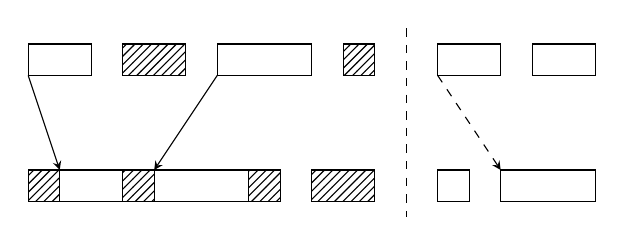
\begin{tikzpicture}[scale=0.4,>=stealth]
    \draw ( 0,4) rectangle +(2,1);
    \draw[pattern=north east lines] ( 3,4) rectangle +(2,1);
    \draw ( 6,4) rectangle +(3,1);
    \draw[pattern=north east lines] (10,4) rectangle +(1,1);
    \draw[pattern=north east lines] ( 0,0) rectangle +(8,1);
    \draw[pattern=north east lines] ( 9,0) rectangle +(2,1);
    \draw[->] (0,4) -- (1,1);
    \draw[->] (6,4) -- (4,1);
    \draw[fill=white] (1,0) rectangle +(2,1);
    \draw[fill=white] (4,0) rectangle +(3,1);
    %
    \draw[dashed] (12,5.5) -- (12,-0.5);
    %
    \draw (13,4) rectangle +(2,1);
    \draw (16,4) rectangle +(2,1);
    \draw (13,0) rectangle +(1,1);
    \draw (15,0) rectangle +(3,1);
    \draw[dashed,->] (13,4) -- (15,1);
  \end{tikzpicture}
  \caption{External calls and memory injections.
    The source and target memory states are
    depicted at the top and bottom
    of the figure. Arrows describe the injection mapping.
    Memory blocks to the right of the dashed line
    have are allocated during the call,
    which adds a new entry to the injection mapping.
    The shaded areas must not be modified by the call.
  }
  \label{fig:injp}
\end{figure}
%}}}

%}}}

\subsection{The \kw{Allocation} pass} %{{{

The \kw{Allocation} pass from \kw{RTL} to \kw{LTL}
is the first pass to modify the interface of function calls.

\kw{LTL} uses \emph{abstract locations}
meant to represent the stack slots and machine registers
used at the assembly level.
Their values are stored in a \emph{location map},
passed across components by the interface $\mathcal{L}$
alongside memory states.
Up to \kw{RTL},
arguments are passed as standalone values,
but in \kw{LTL}
they are mapped to locations.
The compiler also expects the values of
locations designated as \emph{callee-save}
to be preserved by function calls.
This is codified in the $\kw{alloc}$
simulation convention, defined as follows:
\[
  \kw{alloc} := \langle
      \kw{signature} \times \kw{locmap}, \:
      R_\kw{alloc}^\que, \:
      R_\kw{alloc}^\ans \rangle
\]
\[
  \AxiomC{$\vec{v} \vref \kw{args}(sg, ls)$}
  \AxiomC{$m_1 \mext m_2$}
  \BinaryInfC{$
      (sg, rs) \Vdash
      f[sg](\vec{v})@m_1
      \mathrel{R_\kw{alloc}^\que}
      f[sg](ls)@m_2$}
  \DisplayProof
\]
\vspace{0.5ex}
\[
  \AxiomC{$v' \vref \kw{retval}(sg, ls')$}
  \AxiomC{$ls \equiv_\kw{CS} ls'$}
  \AxiomC{$m_1' \mext m_2'$}
  \TrinaryInfC{$
      (sg, ls) \Vdash
      v'@m_1'
      \mathrel{R_\kw{alloc}^\ans}
      ls'@m_2'$}
  \DisplayProof
\]
where $\kw{args}(sg, ls)$ extracts the values of arguments
stored in the location map $ls$ given a function call signature $sg$,
$\kw{retval}(sg, ls)$ likewise extracts the
values returned by the function call, and
$\equiv_\kw{CS}$ relates location maps whose contents agree
on callee-save locations.

%}}}

\subsection{The \kw{Stacking} pass} %{{{

The \kw{Stacking} pass
consolidates the information which
\kw{Linear} stores in abstract stack locations
into the in-memory stack frames of \kw{Mach}.
The simulation uses a memory injection,
and involves maintaining separation properties
ensuring that the source memory and
the various regions of stack frames
are mapped to disjoint areas of the target memory.

With regards to the memory state,
the \kw{stacking} simulation convention
is essentially identical to \kw{injp}.
Since all new sections of stack frames
are outside the image of source memory,
and most of them are local to
their function activation,
the properties of \kw{injp}
are largely sufficient for the proof.

The exception to the rule pertains to argument passing.
Reads from a function's argument locations
access the caller's stack frame.
The \kw{stacking} simulation convention
asserts that the values of argument locations
are indeed stored into corresponding stack slots
within the target memory,
and additionally
requires that the region of the target memory
used to store arguments within the caller's stack
must be disjoint from the injection image of the source memory.

%}}}

\subsection{The \kw{Asmgen} pass} %{{{

\kw{Asm} introduces explicit
program counter, stack pointer and return address registers.
The \kw{Asmgen} pass from \kw{Mach} to \kw{Asm}
uses the following simluation convention:
\begin{gather*}
  \kw{asmgen} := \langle \kw{val} \times \kw{val},
    R_\kw{asmgen}^\que, R_\kw{asmgen}^\ans \rangle
  \\[1ex]
  \AxiomC{$\mathit{rs}_1 \uplus
    [\kw{sp} := \mathit{sp}, \kw{ra} := \mathit{ra}, \kw{pc} := f]
    \vref \mathit{rs}_2$}
  \AxiomC{$m_1 \mext m_2$}
  \BinaryInfC{
    $(\mathit{sp}, \mathit{ra}) \Vdash
     f(\mathit{sp}, \mathit{ra}, \mathit{rs}_1)@m_1
     \mathrel{R_\kw{asmgen}^\que}
     \mathit{rs}_2@m_2$}
  \DisplayProof
  \\[1ex]
  \AxiomC{$
    \mathit{rs}_1' \uplus [\kw{sp} := \mathit{sp}, \kw{pc} := \mathit{ra}]
    \vref \mathit{rs}_2'$}
  \AxiomC{$m_1' \mext m_2'$}
  \BinaryInfC{$
    (\mathit{sp}, \mathit{ra}) \Vdash \mathit{rs}_1'@m_1'
    \mathrel{R_\kw{asmgen}^\ans}
    \mathit{rs}_2'@m_2'$}
  \DisplayProof
\end{gather*}

%}}}

\subsection{Discussion} %{{{

Our use of the \kw{injp}, \kw{alloc} and \kw{stacking}
simulation conventions in particular
underscores the benefits of our approach.
The corresponding passes are the root of
much complexity
in Compositional CompCert, CompCertX and CompCertM.

For instance,
to express the requirement on
the areas protected by \kw{injp},
both CompCompCert and CompCertM
introduce general mechanisms for tracking ownership of
different regions of memory
as part of an extended notion of memory injection.
The approach taken here demonstrates that
the requirements placed on external functions
by the original CompCert
are already good enough for the job!
Because our framework is expressive enough to capture them,
the corresponding passes barely need any modifications,
and the associated issues are resolved before they even show up.

Likewise, the preservation of callee-save registers
ensured by the \kw{Allocation} pass,
and the subtle issues associated with argument-passing
in the \kw{Stacking} pass
have been the cause of much pain
in previous CompCert extensions.
The ease with which they are addressed here
demonstrates the power of
an explicit treatment of abstraction,
made possible
by our notions of language interface and simulation convention.

%The argument passing mechanism has been a source of challenges
%in previous work like Compositional CompCert and CompCertX,
%however it is very straightforward to address
%in our relational, typed framework.
%
%This makes the \kw{Stacking} pass
%much easier to update than in existing work.
%The modest increase in the size of the proof
%comes from the necessity to strenghten
%some invariants the proof keeps track of
%in order to satisfy the incoming simulation convention.

%}}}

%}}}

\section{End-to-end compiler correctness} \label{sec:simalg} %{{{

We now describe the way in which
the simulation proofs of CompCertO
are combined into
a whole-compiler simulation.

\subsection{Simulation convention refinement} %{{{

The core of our simulation algebra is
a notion of refinement for simulation conventions.
The refinement relation $\mathbb{R} \scref \mathbb{S}$
captures the idea that the convention $\mathbb{R}$
is more general than the convention $\mathbb{S}$,
so that any simulation accepting $\mathbb{R}$ as its
incoming convention will accept $\mathbb{S}$ as well.

\begin{definition}[Simulation convention refinement] %{{{
Given two simulation conventions
$\mathbb{R}, \mathbb{S} : A_1 \Leftrightarrow A_2$,
we say that
$\mathbb{S}$ refines $\mathbb{R}$ and write
$\mathbb{R} \scref \mathbb{S}$
when the following holds:
\[
    \begin{array}{r@{}c@{\:\Rightarrow\:}c@{}c@{}l}
      \forall w \,.\, m_1 \, m_2 \,.\, &
      w \Vdash m_1 \mathrel{R^\que} m_2 &
      \exists \, v \,.\, &
      v \Vdash m_1 \mathrel{S^\que} m_2 &
      \: \wedge \\
      \forall \, n_1 \, n_2 \,.\, &
      v \Vdash n_1 \mathrel{S^\ans} n_2 &
      &
      w \Vdash n_1 \mathrel{R^\ans} n_2 & \,.
    \end{array}
\]
We write $\mathbb{R} \equiv \mathbb{S}$ when both
$\mathbb{R} \scref \mathbb{S}$ and
$\mathbb{S} \scref \mathbb{R}$.
\end{definition}
%}}}

The following theorem states the relationship between
simulation convention refinement and forward simulations.

\begin{theorem} %{{{
For
$\mathbb{R}' \scref \mathbb{R} : A_1 \Leftrightarrow A_2$ and
$\mathbb{S} \scref \mathbb{S}' : B_1 \Leftrightarrow B_2$,
the following holds for all
$L_1 : A_1 \rightarrow B_1$ and $L_2 : A_2 \rightarrow B_2$:
\[
      L_1 \le_{\mathbb{R} \rightarrow \mathbb{S}} L_2
      \: \Rightarrow \:
      L_1 \le_{\mathbb{R}' \rightarrow \mathbb{S}'} L_2 \,.
\]
\begin{proof}
See \texttt{open\_fsim\_ccref} in \texttt{CallconvAlgebra.v}.
\end{proof}
\end{theorem}
%}}}

%}}}

\subsection{Composing passes} %{{{

The most basic way to combine simulation proofs
is the notion of vertical composition outlined below.

\begin{definition}[Composition of simulation conventions] %{{{
Given the language interfaces $A_1, A_2, A_3$
and the simulation conventions
$\mathbb{R} : A_1 \Leftrightarrow A_2$ and
$\mathbb{S} : A_2 \Leftrightarrow A_3$,
the composite simulation convention
$\mathbb{R} \cdot \mathbb{S} : A_1 \Leftrightarrow A_3$ is defined as:
\[
    \mathbb{R} \cdot \mathbb{S} :=
      \langle
        W_R \times W_S, \:
        R^\que \cdot S^\que, \:
        R^\ans \cdot S^\ans
      \rangle \,.
\]
\end{definition}
%}}}

\begin{theorem}[Composition of simulations] \label{thm:simcomp} %{{{
For the transition systems
$L_1 : A_1 \rightarrow B_1$,
$L_2 : A_2 \rightarrow B_2$,
$L_3 : A_3 \rightarrow B_3$,
and the simulation conventions
$\mathbb{R}_A : A_1 \Leftrightarrow A_2$,
$\mathbb{R}_B : B_1 \Leftrightarrow B_2$,
$\mathbb{S}_A : A_2 \Leftrightarrow A_3$, and
$\mathbb{S}_B : B_2 \Leftrightarrow B_3$,
the following holds:
\[
  \AxiomC{$L_1 \le_{\mathbb{R}_A \rightarrow \mathbb{R}_B} L_2$}
  \AxiomC{$L_2 \le_{\mathbb{S}_A \rightarrow \mathbb{S}_B} L_3$}
  \BinaryInfC{
    $L_1 \le_{\mathbb{R}_A \cdot \mathbb{S}_A \rightarrow
                   \mathbb{R}_B \cdot \mathbb{S}_B} L_3$}
  \DisplayProof
\]
\begin{proof}
\texttt{compose\_open\_fsim} in \texttt{common/Smallstep.v}.
\end{proof}
\end{theorem}
%}}}

\begin{theorem} % assoc, id, monot {{{
For
$\mathbb{R} : A_1 \Leftrightarrow A_2$,
$\mathbb{S} : A_2 \Leftrightarrow A_3$,
$\mathbb{T} : A_3 \Leftrightarrow A_4$,
the following properties hold:
\begin{gather*}
  ({\cdot}) :: {{\scref} \times {\scref} \rightarrow {\scref}}
  \\
  (\mathbb{R} \cdot \mathbb{S}) \cdot \mathbb{T} \equiv
    \mathbb{R} \cdot (\mathbb{S} \cdot \mathbb{T})
  \qquad
  \mathbb{R} \cdot \kw{id} \equiv
  \kw{id} \cdot \mathbb{R} \equiv
  \mathbb{R}
\end{gather*}
\end{theorem}
%}}}

%}}}

\subsection{Simplifying simulation conventions} %{{{

Using the constructions presented so far,
we can define:
\[
    \mathbb{C}^\flat :=
      \kw{alloc} \cdot
      \kw{ext}_\mathcal{L} \cdot
      \kw{stacking} \cdot
      \kw{asmgen}
\]
and compose the passes \kw{Allocation}--\kw{Asmgen}
to get a simulation of type
$\mathbb{C}^\flat \twoheadrightarrow \mathbb{C}^\flat$.
Going further,
refinement and composition allow us to formulate
properties of \kw{inj} and \kw{ext}.

\begin{theorem} \label{thm:extinj}
$
  \kw{ext} \cdot \kw{inj} \equiv
  \kw{inj} \cdot \kw{ext} \equiv
  \kw{inj} \cdot \kw{inj} \equiv
  \kw{inj}
$.
\begin{proof}
\texttt{ext\_inj}, \texttt{inj\_ext}, \texttt{inj\_inj},
found under \texttt{cklr/}.
\end{proof}
\end{theorem}

This make it possible to simplify
the compiler's incoming convention
into $\kw{inj} \cdot \mathbb{C}^\flat$,
but unfortunately \kw{injp}
does not compose with \kw{ext} and itself in the same way.
However, conventions
admit the following Kleene algebra.

\begin{definition} %{{{
Consider $(\mathbb{R}_i)_{i \in I}$
a family of conventions
with
$\mathbb{R}_i = \langle W_i, R_i^\que, R_i^\ans \rangle
  : A_1 \Leftrightarrow A_2$
for all $i \in I$.
The least upper bound
can be defined as
$\sum_{i \in I} \mathbb{R}_i := \langle W, R^\que, R^\ans \rangle$
where:
\[
  W := \sum_{i \in I} W_i  \qquad
  \begin{array}{l}
  (i, w) \Vdash R^\que \: = \: w \Vdash R_i^\que \\[1ex]
  (i, w) \Vdash R^\ans \: = \: w \Vdash R_i^\ans \,.
  \end{array}
\]
We will write $\mathbb{R}_1 + \cdots + \mathbb{R}_n$
for the finitary case $\sum_{i=1}^n \mathbb{R}_i$.
Then for $\mathbb{R} : A_1 \Leftrightarrow A_2$,
we define
$\mathbb{R}^* := \sum_{n \in \mathbb{N}} \mathbb{R}^n$,
where:
\[
  \mathbb{R}^0 := \kw{id} \qquad
  \mathbb{R}^{n+1} := \mathbb{R}^n \cdot \mathbb{R} \,.
\]
\end{definition}
%}}}

These constructions allows us to generalize the compiler's
outgoing simulation convention to
$(\kw{ext} + \kw{injp})^* \cdot \mathbb{C}^\flat$.
The following theorem will also be useful.

\begin{theorem}[Addition and Kleene iteration of simulations] \label{thm:simk} %{{{
The following properties hold:
\[
  \AxiomC{$\forall i \,.\,
    L_1 \le_{\mathbb{R} \rightarrow \mathbb{S}_i} L_2$}
  \UnaryInfC{$
    L_1 \le_{\mathbb{R} \rightarrow \sum_i \mathbb{S}_i} L_2$}
  \DisplayProof
  \quad
  \AxiomC{$L \le_{\mathbb{R} \rightarrow \mathbb{S}} L$}
  \UnaryInfC{$L \le_{\mathbb{R}^* \rightarrow \mathbb{S}^*} L$}
  \DisplayProof
\]
\begin{proof}
See \texttt{cc\_star\_fsim} and the preceding definitions
in \texttt{common/CallconvAlgebra.v}.
\end{proof}
\end{theorem}
%}}}

%}}}

\subsection{Compiler correctness} %{{{

We have simplified both the incoming and outgoing conventions
used by the whole-compiler simulation,
but they remain distinct and incomparable.
To reconcile them,
we will use the following properties
of \kw{Clight} and \kw{RTL}.

\begin{theorem} \label{thm:lprops} %{{{
These simulations hold
for all programs:
\begin{gather*}
\forall \, p \,.\,
  \kw{Clight}(p)
  \le_{(\kw{ext} + \kw{injp})^* \rightarrow (\kw{ext} + \kw{injp})^*}
  \kw{Clight}(p) \\
\forall \, p \,.\,
  \kw{RTL}(p)
  \le_{\kw{inj} \rightarrow \kw{inj}}
  \kw{RTL}(p)
\end{gather*}
\begin{proof}
Using Thm~\ref{thm:param} and \ref{thm:simk}.
\end{proof}
\end{theorem}
%}}}

By introducing these self-simulations
at strategic points in the overall composition of passes
shown in Table~\ref{tbl:passes},
we can finally establish the following correctness theorem.

\begin{theorem}[Compositional Correctness of CompCertO] \label{thm:compc} %{{{
For a \kw{Clight} program $p$
and an \kw{Asm} program $p'$ such that
$\kw{CompCert}(p) = p'$,
the following simulation holds:
\[
    \kw{Clight}(p) \le_{\mathbb{C} \rightarrow \mathbb{C}}
    \kw{Asm}(p') \,,
\]
where $\mathbb{C}$ is the simulation convention defined as:
\[
    \mathbb{C} := (\kw{ext} + \kw{injp})^* \cdot \kw{inj} \cdot
      \mathbb{C}^\flat
%      \kw{alloc} \cdot
%      \kw{ext}_\mathcal{L} \cdot
%      \kw{stacking} \cdot
%      \kw{asmgen} \,.
\]
\begin{proof}
Use Thm.~\ref{thm:simcomp} to compose
the correctness proofs of the compiler passes and
self-simulations shown in Table~\ref{tbl:passes}.
By properties of the Kleene star,
the outgoing simulation convention of each of the
passes \kw{SimplLocals}--\kw{Unusedglob}
can be folded into $(\kw{ext} + \kw{injp})^*$
to obtain the overall outgoing convention $\mathbb{C}$.
Likewise, by Thm.~\ref{thm:extinj}
their incoming simulation conventions
can be folded into $\kw{inj}$
to obtain the overall incoming convention $\mathbb{C}$.
See also \texttt{driver/Compiler.v}.
\end{proof}
\end{theorem}
%%}}}

%}}}

%}}}

\section{Evaluation} \label{sec:eval} %{{{

We now discuss the possible uses of the theorems we have proved,
and the proof effort involved in our development.

\subsection{Compositional compilation and verification} \label{sec:cver} %{{{

Referring back to Fig.~\ref{fig:process},
consider the modules
$\mathtt{M1.c}, \ldots, \mathtt{Mn.c}$
compiled and linked to
$\mathtt{M1.s} \oplus \ldots \oplus \mathtt{Mn.s} = \mathtt{M.s}$,
we can use
Thms.~\ref{thm:asmlinking},
\ref{thm:simlinking} and
\ref{thm:compc}
to establish the following separate compilation property:
\begin{equation}
  \label{eqn:sepcomp}
  \kw{Clight}(\mathtt{M1.c}) \oplus \cdots \oplus \kw{Clight}(\mathtt{Mn.c})
  \le_{\mathbb{C} \twoheadrightarrow \mathbb{C}}
  \kw{Asm}(\mathtt{M.s})
\end{equation}
That is,
the linked \kw{Asm} program
$\mathtt{M.s}$
faithfully implements
the horizontal composition of the source modules' behaviors,
following the simulation convention $\mathbb{C}$.

Additionally,
suppose we wish to verify that the overall program
satisfies a specification $\Sigma$,
also expressed as a transition system
for $\mathcal{C} \twoheadrightarrow \mathcal{C}$.
We must first show that $\Sigma$ can be decomposed
along the lines of the program's components:
\[
    \Sigma \: \le_{\kw{id} \twoheadrightarrow \kw{id}} \:
    \Sigma_1 \oplus \cdots \oplus \Sigma_n \,.
\]
Then for each module, we prove that
$\Sigma_i \le_\kw{id} \kw{Clight}(\mathtt{Mi.c})$.
This can be combined with Thm.~\ref{thm:simlinking} and Eqn.~\ref{eqn:sepcomp}
to establish:
\[
    \Sigma \le_{\mathbb{C} \twoheadrightarrow \mathbb{C}} \kw{Asm}(\mathtt{M.s}) \,.
\]

Note that Eqn.~\ref{eqn:sepcomp} can be established
as long as the property
$\kw{Clight}(\mathtt{Mi.c})
 \le_{\mathbb{C} \twoheadrightarrow \mathbb{C}}
 \kw{Asm}(\mathtt{Mi.s})$
holds independently for each module.
It is possible for the different $\mathtt{Mi.s}$
to be obtained by different compilers,
as long as each one satisfies a correctness property
following the simulation convention in Thm.~\ref{thm:compc}.
Indeed this is the case of the versions of CompCertO
obtained by enabling different optimization passes.

Going one step further,
as presented our framework supports linking
with assembly modules in the following, limited sense.
If some of the components $\mathtt{Mi.s}$
are a hand-written and
satisfy C-style specifications $\Sigma_i$,
then we can prove on a case-by-case basis that
$\Sigma_i \le_{\mathbb{C} \twoheadrightarrow \mathbb{C}} \kw{Asm}(\mathtt{Mi.s})$
and proceed with the rest of the proof as before.
In the case of assembly modules
whose behavior cannot be described
by the $\mathcal{C}$ language interface,
it may still be possible to exploit the compiler's
correctness theorem
to characterize the behavior of the components
compiled from C
in an ad-hoc proof about the behavior of the linked
assembly program.
However, the framework we have presented
does not provide a systematic way
to represent or manipulate
such a configuration.

%}}}

\subsection{Proof effort} \label{sec:effort} %{{{

\begin{table} % tbl:slocs {{{
  \begin{tabular}{lr@{\:}r}
    \hline
    Component & SLOC & \\ %\multicolumn{2}{r}{SLOC} \\
    \hline
    Semantic framework (\S\ref{sec:sem}) & $+1079$ & ($20\%$) \\
    Correctness proofs (\S\ref{sec:passes}) & $\approx$+600 & (5\%) \\
    CKLR theory and instances (\S\ref{sec:cklrdef}) & $1{,}807$ & \\
    \kw{Clight} and \kw{RTL} parametricity (\S\ref{sec:param}) & $2{,}702$ & \\
    Simulation convention algebra (\S\ref{sec:simalg}) & $998$ & \\
    \hline
  \end{tabular}
  \caption{Significant lines of code in CompCertO
    relative to CompCert v$3.5$.
    See also Table~\ref{tbl:passes}
    for a per-pass breakdown of the correctness proofs.}
  \label{tbl:slocs}
\end{table}
%}}}

To give a sense of the overall complexity of CompCertO,
we list in Table~\ref{tbl:slocs}
the increase in significant lines of code it introduces
compared to CompCert v$3.5$.
As discussed in \S\ref{sec:passes},
our methodology comes with only a very modest increase
in the complexity of most passes.

Although SLOC is an imperfect measure,
and a 1:1 comparison between developments which
prove different things is difficult,
our numbers represent
a drastic improvement over Compositional CompCert,
and compare favorably
or are on par with
the corresponding sections of CompCertM.

%}}}

%}}}

\section{Related work} \label{sec:rw} %{{{

Patterson and Ahmed provide a general survey,
discussion and synthesis of various
compositional compiler correctness results in \cite{next700}.
We focus here on extensions to CompCert
and how they relate to our own.

The conceptual framework of game semantics
can be used to classify previous work
on semantic models of CompCert.
By reinterpreting these models
in terms of games and strategies,
we can establish the taxonomy presented in
Table~\ref{tbl:compcerts}.

\begin{table} % tbl:compcerts {{{
  \begin{tabular}{lc}
    \hline
    Variant & Semantic model \\
    \hline
    (Sep)CompCert \cite{compcert,sepcompcert} &
      $\chi : \mathbf{1} \twoheadrightarrow \mathcal{C}
       \vdash \mathbf{1} \twoheadrightarrow \mathcal{W}$ \\
    CompCertX \cite{popl15} &
      $\chi : \mathbf{1} \twoheadrightarrow \mathcal{C} \vdash
       \mathbf{1} \twoheadrightarrow \mathcal{C}$ \\
    CompCompCert \cite{compcompcert} &
      $\mathcal{C} \rightarrow \mathcal{C}$ \\
    CompCertM \cite{compcertm} &
      $\mathcal{C} \times \mathcal{A} \twoheadrightarrow
       \mathcal{C} \times \mathcal{A}$ \\
    CompCertO &
      $A \twoheadrightarrow A \quad
      (A \in \{\mathcal{C}, \mathcal{L}, \mathcal{M}, \mathcal{A}\})$ \\
    \hline
  \end{tabular}
  \vspace{1ex}
  \caption{Taxonomy of extensions to CompCert semantics.
    The parameter $\chi : \mathbf{1} \twoheadrightarrow \mathcal{C}$
    pre-specifies the behavior of external functions,
    whereas games on the left of arrows
    correspond to dynamic interactions.
    %The CompCertO model
    %is parametrized by the languages interfaces $A$, $B$.
  }
  \label{tbl:compcerts}
\end{table}
%}}}

\paragraph{CompCert and SepCompCert} %{{{

As noted in \S\ref{sec:mainideas:compcerto},
the whole-program semantics used by CompCert
express strategies for the game
$\mathbf{1} \twoheadrightarrow \mathcal{W}$.
CompCert's original correctness theorem
stated the refinement property
$\kw{C}_\mathcal{W}(p) \sqsubseteq \kw{Asm}_\mathcal{W}(p')$,
where $\kw{C}_\mathcal{W}$ and $\kw{Asm}_\mathcal{W}$
denote the source and target whole-program semantics.
This was later extended by SepCompCert \cite{sepcompcert},
which introduced the linking operator $+$
and generalized the correctness theorem to
the form discussed in \S\ref{sec:sem:overview}.
%Our work uses the same notion of linking
%for target \kw{Asm} programs.

Since the semantic model does not account
for external calls,
they are interpreted %in every language semantics
using a common global parameter $\chi$
specifying their behavior.
The correctness proof assumes that $\chi$ is deterministic
and that it satisfies a number of healthiness requirements
with respect to the memory transformations
used in CompCert's correctness proof,
corresponding roughly to self-simulation
under the CKLR $\kw{ext}$ and $\kw{injp}$.

%}}}

\paragraph{Contextual compilation} %{{{

CompCertX \cite{popl15} generalizes
the incoming interface of programs
from $\mathcal{W}$ to $\mathcal{C}$,
and as such charaterizes the behavior
not only of \texttt{main}
but of any function of the program,
called with any argument values.

This allows CompCertX and its correctness theorem
to be used in the layer-based verification of
the CertiKOS kernel:
once the code of a given abstraction layer has been verified
and compiled using CompCertX,
that layer's specification can be used as the new $\chi$
when the next layer is verified.
%This enabled the verification of CertiKOS ---
%an artifact of significant size ---
%at the level of assembly code,
%by integrating CompCert as part of its proof of correctness.
However,
this approach does not support two-way invocations between components,
and requires the healthiness conditions on $\chi$
to be proved before the next layer is added.

%}}}

\paragraph{Compositional CompCert} %{{{

The \emph{interaction semantics} of
Compositional CompCert \cite{compcompcert}
are closer to our own model
but are limited to the language interface $\mathcal{C}$.
Likewise, the simulations used in Compositional CompCert
correspond to our notion of forward simulation
for a single convention called \emph{structured injections},
which we will write $\mathbb{SI}$.
Simulation proofs are updated to follow this model,
and the \emph{transitivity} of $\mathbb{SI}$ is established
($\mathbb{SI} \cdot \mathbb{SI} \scref \mathbb{SI}$),
so that passes can be composed
to obtain a simulation for the whole compiler.

Compositional CompCert also introduced a notion of \emph{semantic linking}
similar to our horizontal composition
(\S\ref{sec:sem:linker}).
As in our case,
semantic linking is shown to preserve simulations
(Thm.~\ref{thm:simlinking}),
however semantic linking is not related to
syntactic linking of assembly programs,
and this was later shown to be problematic \cite{compcertm}.

Another limitation of Compositional CompCert
is the complexity of the theory
and the proof effort required.
Because of the use of a single simulation convention,
many assumptions naturally expressed as
relational invariants in the simulation relations of CompCert
must be either captured by $\mathbb{SI}$
or handled at the level of language semantics,
and simulation proofs
essentially had to be rewritten and adapted to
structured injections.

%}}}

\paragraph{CompCertM} %{{{

The most recent extension of CompCert is CompCertM \cite{compcertm},
which shares common themes and was developped concurrently
with our work.

The module semantics of CompCertM
builds on interaction semantics
by incorporating an assembly language interface.
The resulting semantic model can be characterized as
$\mathcal{C} \times \mathcal{A} \twoheadrightarrow
 \mathcal{C} \times \mathcal{A}$.
The simulations used to verify passes
are parametrized by Kripke relations similar to CKLRs.
While these do not directly compose,
a new technique called \emph{refinement under self-related context}
(RUSC)
can nonetheless be used to derive a contextual refinement theorem
for the whole compiler with only minimal overhead.

This approach has many advantages.
CompCertM avoids much of the complexity
of Compositional CompCert
when it comes to composing passes,
and the flexibility of the simulations used
makes updating the correctness proofs of passes much easier.
CompCertM also charts new ground in several directions.
The RUSC relation used to state the final theorem
is shown to be adequate with respect to the trace semantics
of closed programs.
CompCertM has improved support for static variables
and module-local state,
can be used to carry out compositional verification,
and the verification of
the assembly runtime function \texttt{utod} is demonstrated.

In other aspects,
CompCertM inherits the limitation of previous approaches
whereas CompCertO goes a step further.
Because the compiler correctness theorem
is not itself expressed as a simulation,
it fails requirement \#\ref{req:opensim}
laid out in \S\ref{sec:compcertreq}.
While it may be possible to accomodate \#\ref{req:openabs},
the parametrization of simulations
does not offer the same flexibility as
our full-blown notion of simulation convention.
As a consequence, a cascade of techniques
(\emph{repaired} interaction semantics,
\emph{enriched} memory injections,
the mixed simulations of \cite{pilsner})
need to be deployed to enforce invariants
which find a natural relational expression
under our appoach.

Therefore,
an interesting question for future investigation
will be to determine to what extent
the techniques used by CompCertM and CompCertO
could be integrated to combine
the relative strengths of both developments.

%}}}

%\vspace{2em}
%[Somewhere?]
%Embracing the difference between the interfaces of
%the source and target languages
%represents a significant departure from established practice.
%Existing work goes great lengths
%to ensure that the source and target semantics
%are expressed in the same semantic domain.
%Indeed,
%the success of CompCert itself
%relies in part on its use of a flexible
%but uniform memory model,
%capable both of modeling the C standard accurately,
%and of giving a reasonable account
%of assembly-level mechanics.
%Later work such as \cite{compcompcert,cpp15}
%follows this precedent and uses
%a uniform interface for open modules,
%and treats source and target calls
%as essentially the same,
%and ensuring that any differences introduced by the compiler
%are absorbed by a semantic framework
%defined \emph{modulo} memory transformations.

%}}}

\bibliographystyle{abbrv}
\bibliography{lwcc}

\end{document}
